\PassOptionsToPackage{obeyspaces,spaces,hyphens}{url}
\documentclass{SBCbookchapter}
\usepackage[utf8]{inputenc}
\usepackage[T1]{fontenc}
\usepackage[english,brazilian]{babel}
\usepackage{graphicx}
\usepackage{array}
\usepackage{booktabs}
\usepackage{longtable}
\usepackage{tabularx}
\usepackage{multirow}
\usepackage{xcolor}
\usepackage{listings}
\usepackage{pdflscape}
\usepackage{placeins}
\usepackage{tikz}
\usetikzlibrary{shapes.geometric,positioning}
\usepackage{url}
\usepackage[hidelinks]{hyperref}
\usepackage{microtype}

\graphicspath{{figuras/}}

\makeatletter
% Legendas de longtable no mesmo estilo do modelo SBC (Helvetica 10 pt, negrito)
\def\LT@makecaption#1#2#3{%
  \LT@mcol\LT@cols c{\hbox to\z@{\hss\parbox[t]\LTcapwidth{%
    \centering\sffamily\captionsize\textbf{#2. #3}\par\vskip\belowcaptionskip}\hss}}}
\makeatother
\setlength{\LTcapwidth}{\textwidth}
\setlength{\LTpre}{6pt}
\setlength{\LTpost}{6pt}

\newcommand{\pendente}[1]{\textcolor{red}{\textbf{[PENDENTE: #1]}}}
\newcommand{\repo}{\url{https://github.com/lipe0312/eventos-mata60}}
\DeclareUrlCommand\cod{\urlstyle{tt}}
\makeatletter
\g@addto@macro\UrlBreaks{\do\_\do\(\do\)\do\,}
\Urlmuskip=0mu plus 2mu
\makeatother
\newcolumntype{L}[1]{>{\raggedright\arraybackslash}p{#1}}
\newcolumntype{Y}{>{\raggedright\arraybackslash}X}

\lstdefinestyle{sql}{
  language=SQL,
  basicstyle=\ttfamily\footnotesize,
  keywordstyle=\bfseries,
  columns=fullflexible,
  keepspaces=true,
  frame=tb,
  framerule=0.4pt,
  aboveskip=6pt,
  belowskip=6pt,
  showstringspaces=false,
  breaklines=true,
  morekeywords={GENERATED,ALWAYS,IDENTITY,DEFERRABLE,INITIALLY,DEFERRED,TRIGGER,EXECUTE,FUNCTION,RECURSIVE,ATOMIC,PROCEDURE,ROLE,GRANT,USAGE,SCHEMA}
}
\lstset{style=sql}

\renewcommand{\arraystretch}{1.15}

% Figuras do MER, já recortadas em PDF vetorial e nomeadas pelo número no relatório.
% Foram geradas a partir das exportações do brModelo (mer-final.pdf, VF2, e mer-v1.pdf),
% com trim = esquerda inferior direita superior, em pontos:
%   figura-1-2-mer-v1        28 30 28 30            (mer-v1)
%   figura-1-3-mer-geral     35 36 83 36            (mer-final)
%   figura-1-4-mer-parte-a   26.2 37.3 547.4 281.5  (mer-final)
%   figura-1-5-mer-parte-b   278.2 68.1 220.1 278.2 (mer-final)
%   figura-1-6-mer-parte-c   49.1 303.7 357.6 68.7  (mer-final)
%   figura-1-7-mer-parte-d   428.7 192.4 114.1 94.9 (mer-final)
%   figura-1-8-mer-parte-e   526.9 225.1 76.1 32.7  (mer-final)
%   figura-1-9-mer-parte-f   418.9 37.3 76.1 402.5  (mer-final)
\newcommand{\mervum}{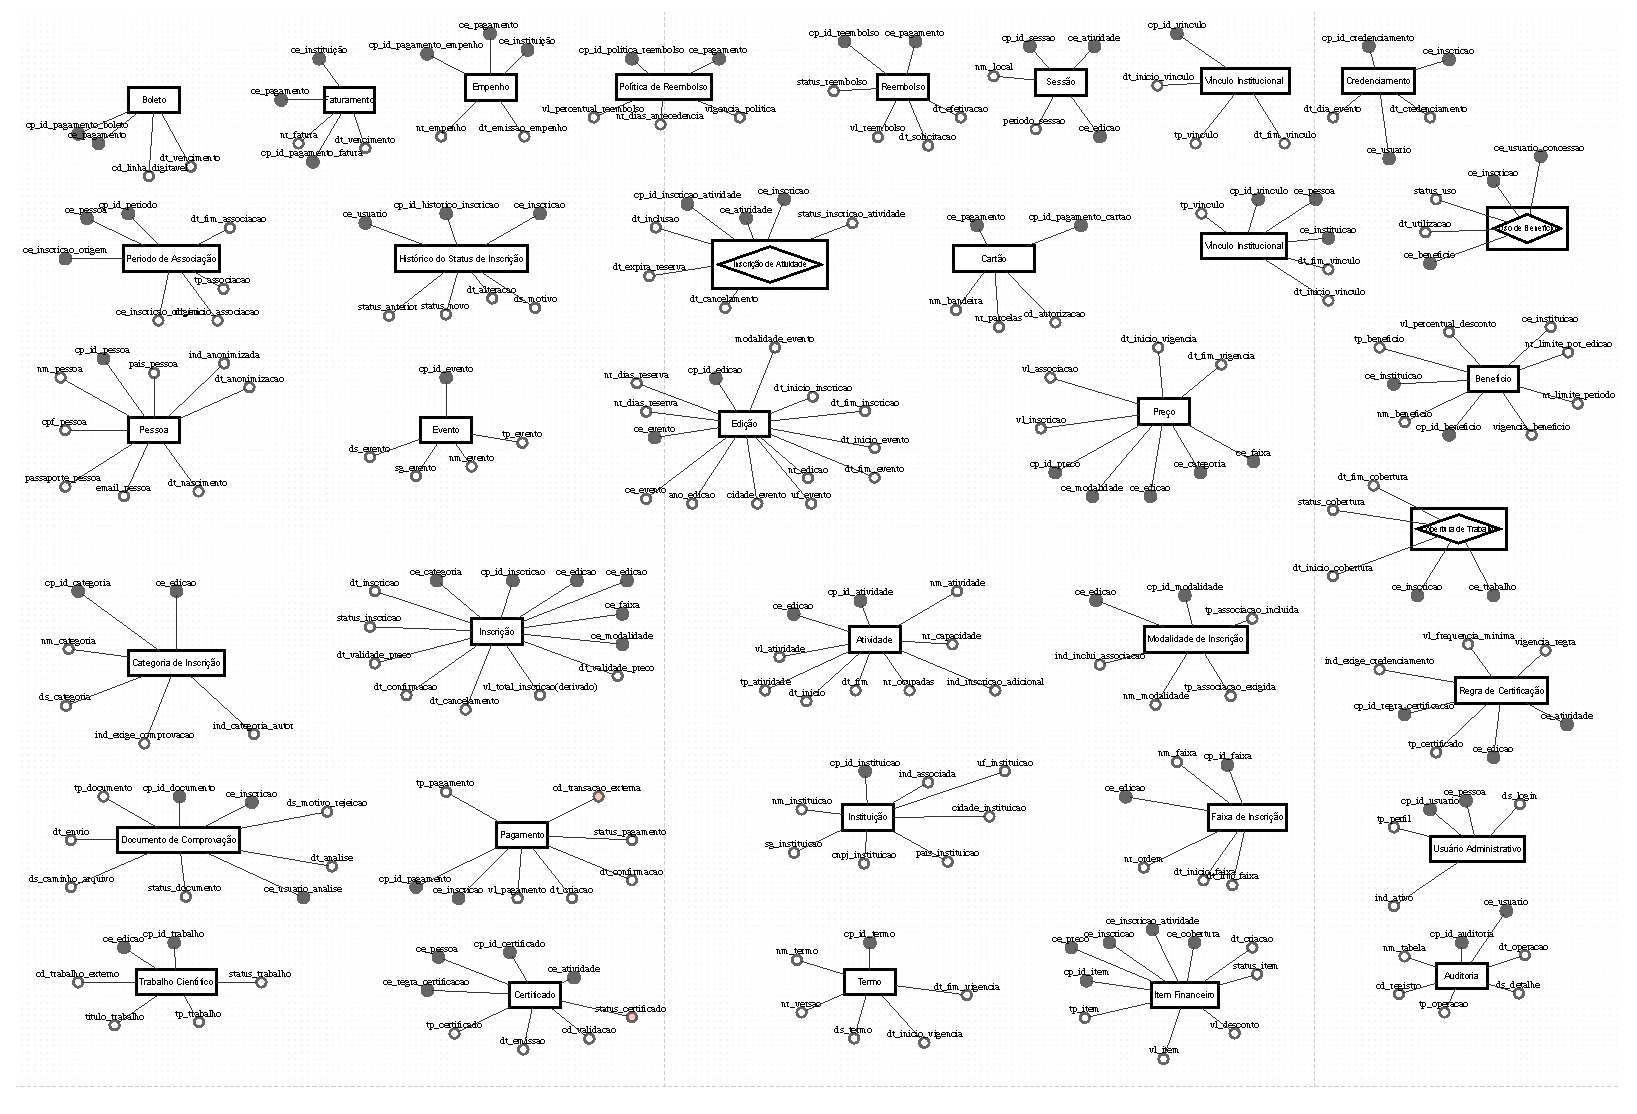
\includegraphics[width=\linewidth]{figura-1-2-mer-v1}}
\newcommand{\mergeral}{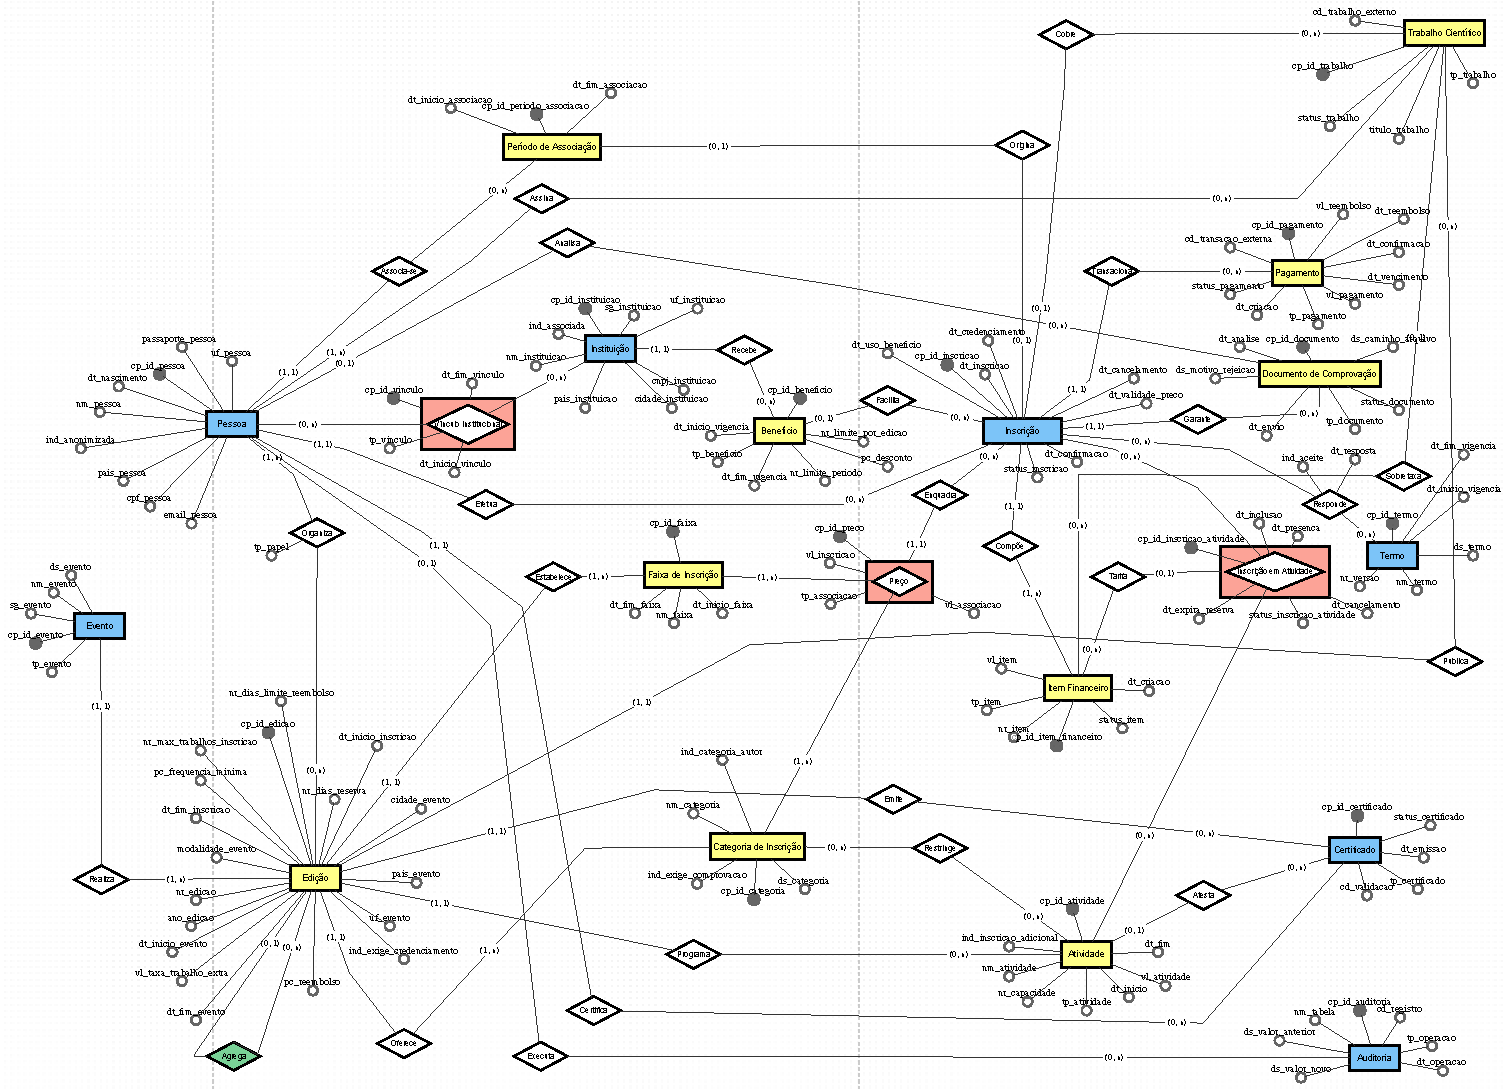
\includegraphics[width=\linewidth,height=0.97\textheight,keepaspectratio]{figura-1-3-mer-geral}}
\newcommand{\merA}{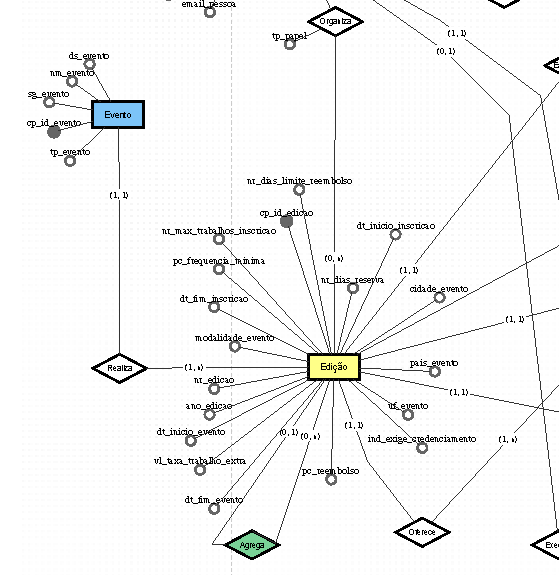
\includegraphics[width=0.78\linewidth]{figura-1-4-mer-parte-a}}
\newcommand{\merB}{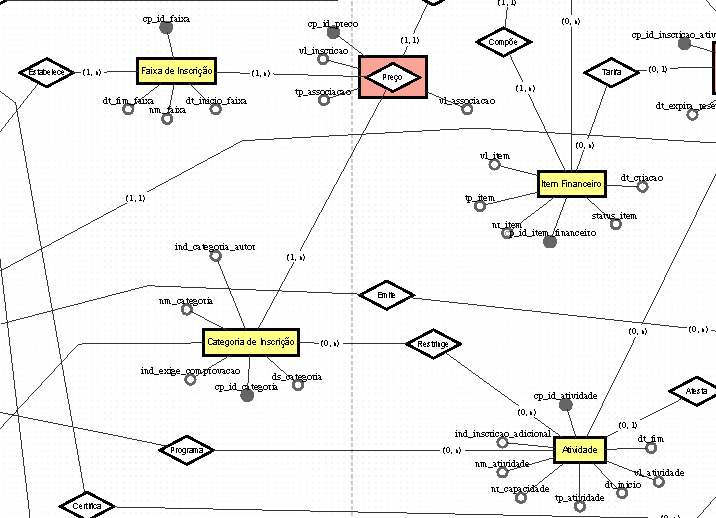
\includegraphics[width=\linewidth]{figura-1-5-mer-parte-b}}
\newcommand{\merC}{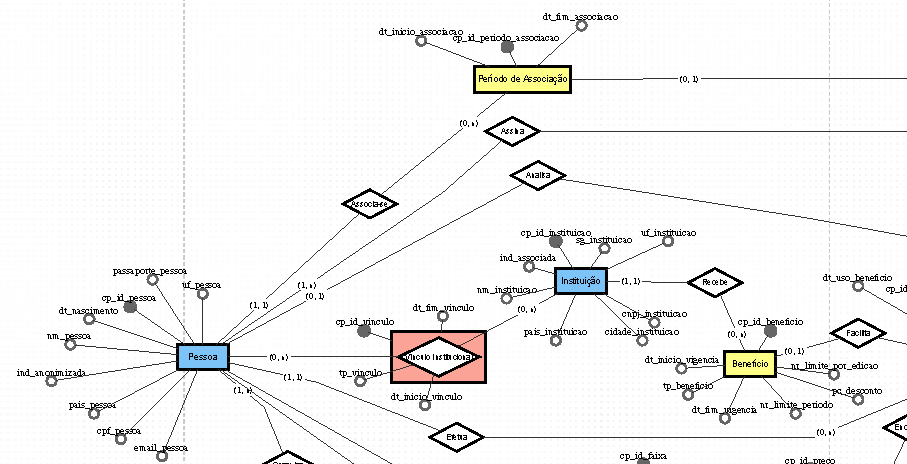
\includegraphics[width=\linewidth]{figura-1-6-mer-parte-c}}
\newcommand{\merD}{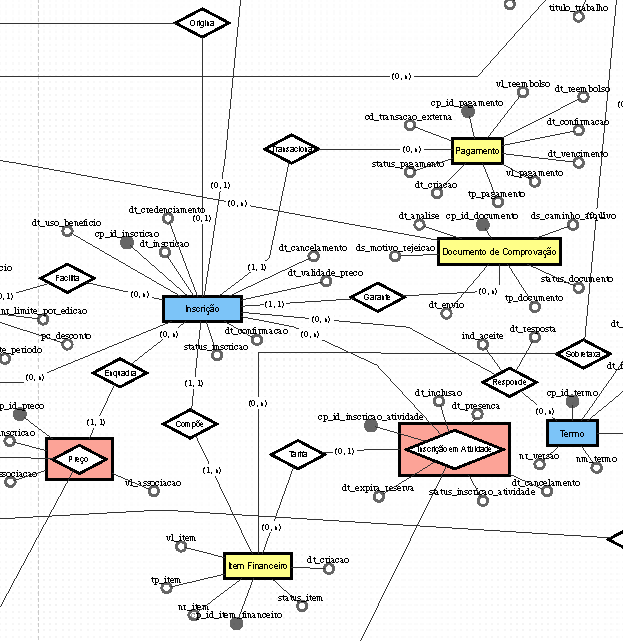
\includegraphics[width=0.9\linewidth]{figura-1-7-mer-parte-d}}
\newcommand{\merE}{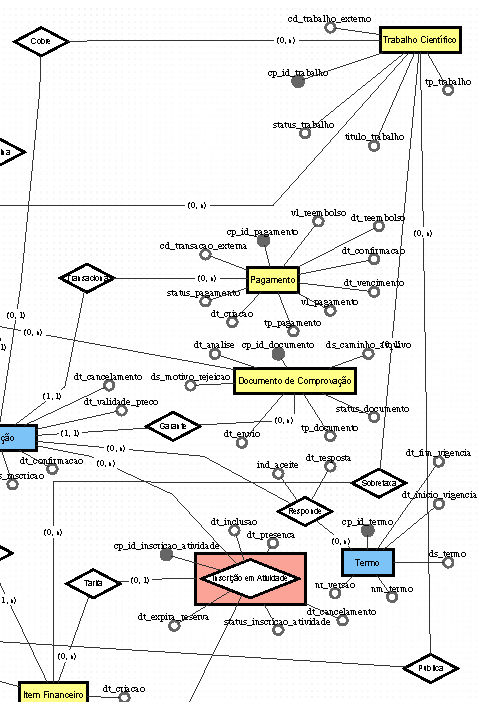
\includegraphics[width=0.7\linewidth]{figura-1-8-mer-parte-e}}
\newcommand{\merF}{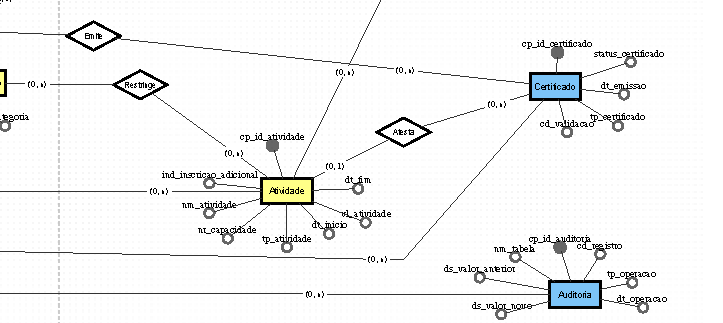
\includegraphics[width=\linewidth]{figura-1-9-mer-parte-f}}

% Figuras do modelo lógico, recortadas de logico-final.pdf (exportação VF do brModelo), trim em pontos:
%   figura-1-10-logico-geral    34 36 187 35
%   figura-1-11-logico-parte-a  32.7 297.1 573.6 49.1
%   figura-1-12-logico-parte-b  219.3 346.2 380.5 68.7
%   figura-1-13-logico-parte-c  45.8 85.7 645.6 297.8
%   figura-1-14-logico-parte-d  265.1 143.3 370.6 288.0
%   figura-1-15-logico-parte-e  209.5 32.1 344.5 441.8
%   figura-1-16-logico-parte-f  448.4 280.8 190.6 32.7
%   figura-1-17-logico-parte-g  490.9 149.9 187.4 343.6
\newcommand{\loggeral}{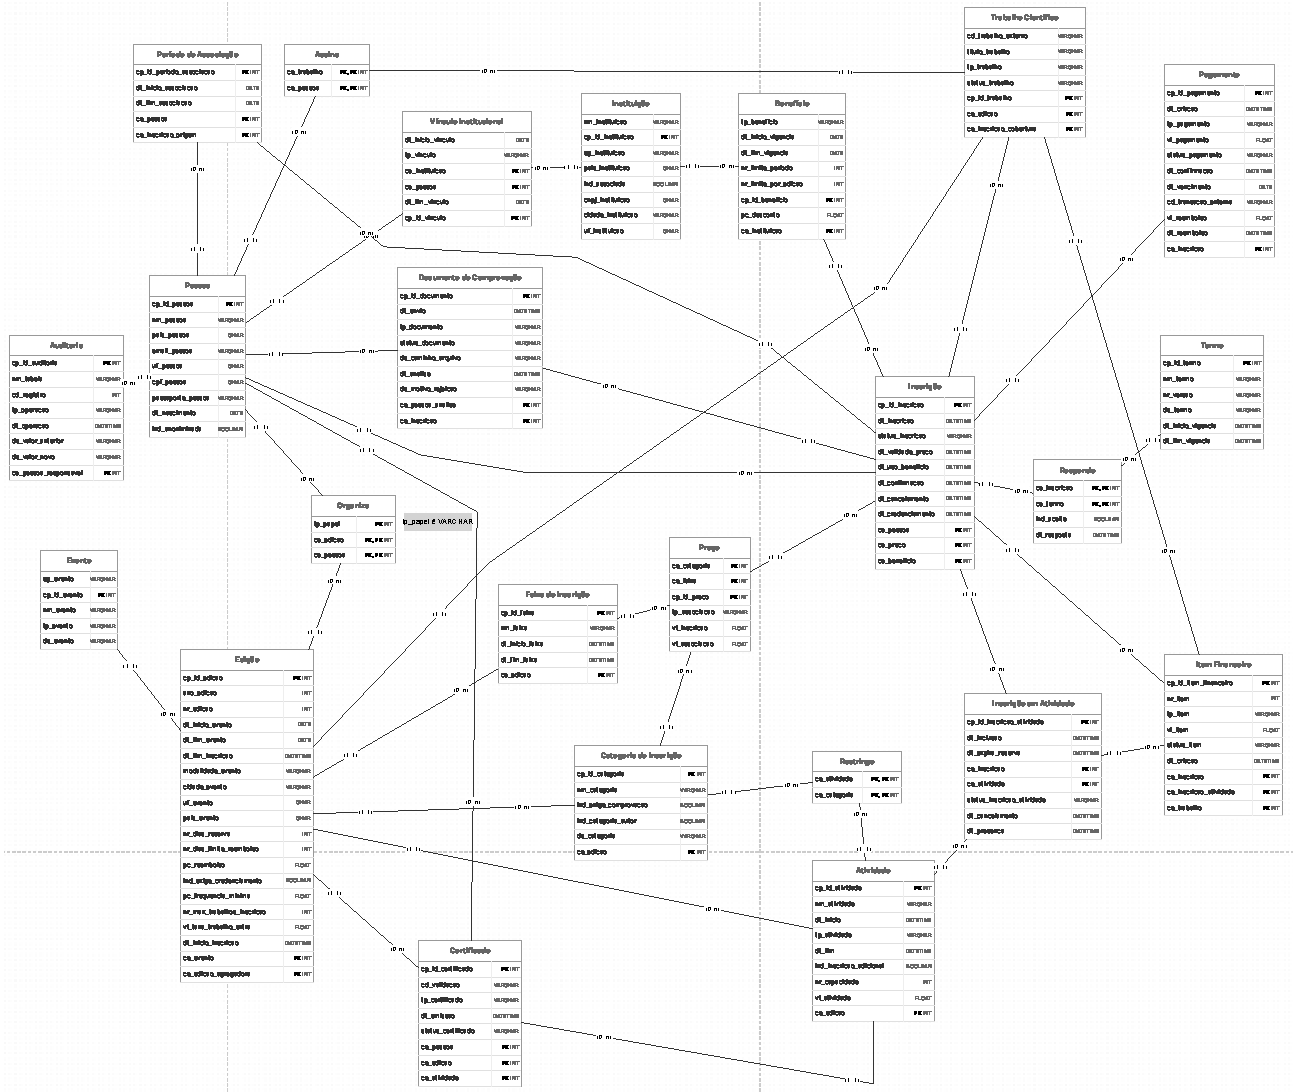
\includegraphics[width=\linewidth,height=0.97\textheight,keepaspectratio]{figura-1-10-logico-geral}}
\newcommand{\logA}{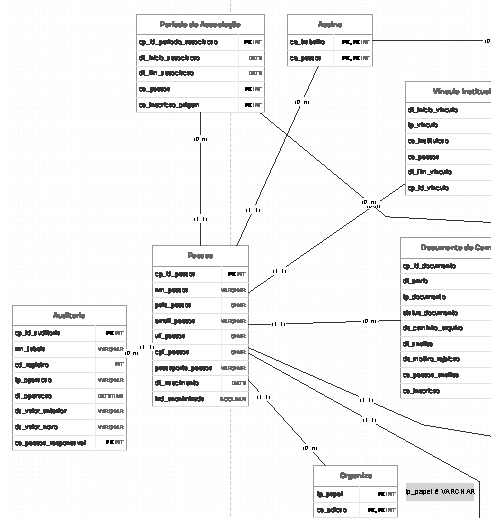
\includegraphics[width=0.95\linewidth]{figura-1-11-logico-parte-a}}
\newcommand{\logB}{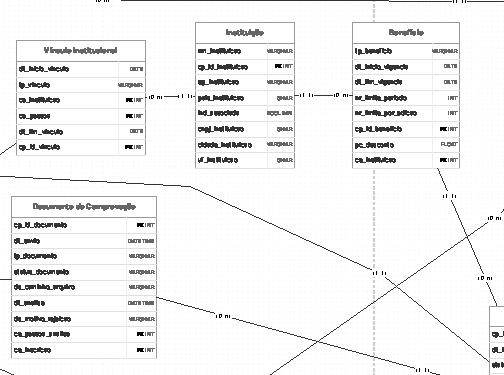
\includegraphics[width=\linewidth]{figura-1-12-logico-parte-b}}
\newcommand{\logC}{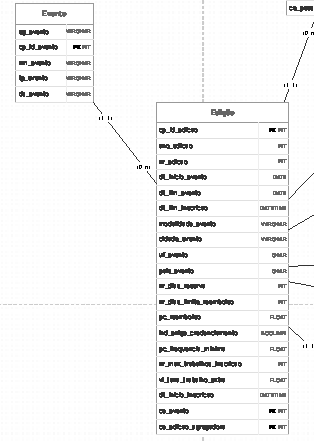
\includegraphics[width=0.6\linewidth]{figura-1-13-logico-parte-c}}
\newcommand{\logD}{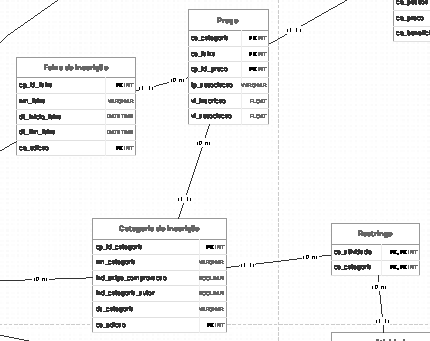
\includegraphics[width=0.82\linewidth]{figura-1-14-logico-parte-d}}
\newcommand{\logE}{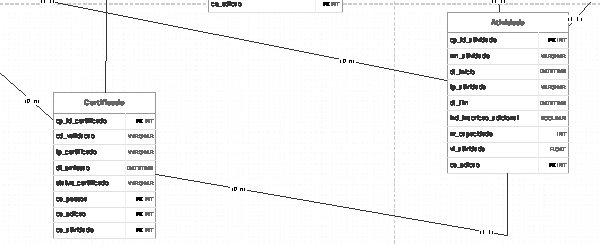
\includegraphics[width=\linewidth]{figura-1-15-logico-parte-e}}
\newcommand{\logF}{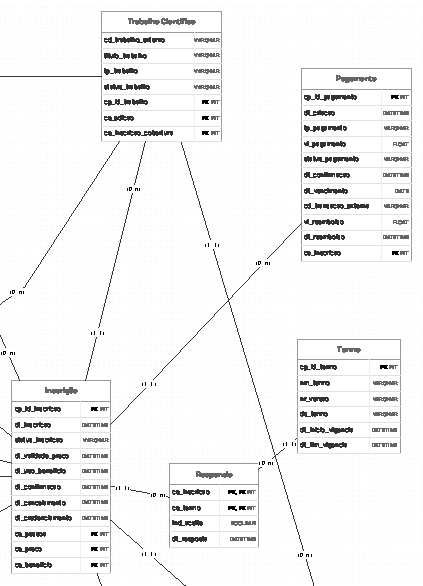
\includegraphics[width=0.8\linewidth]{figura-1-16-logico-parte-f}}
\newcommand{\logG}{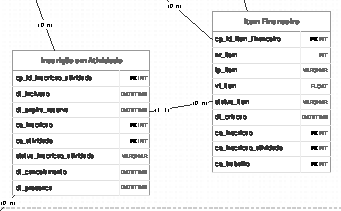
\includegraphics[width=0.66\linewidth]{figura-1-17-logico-parte-g}}

% Cores do brModelo, medidas na exportação do diagrama
\definecolor{brforte}{HTML}{7CC4F8}
\definecolor{brfraca}{HTML}{FFFF88}
\definecolor{brassoc}{HTML}{FCA397}
\definecolor{brauto}{HTML}{79D297}
\definecolor{brrel}{HTML}{F9F9F9}
\definecolor{bratrib}{HTML}{666666}
\tikzset{
  ent/.style={draw=black,line width=0.9pt,minimum width=1.9cm,minimum height=0.62cm,font=\sffamily\scriptsize},
  rel/.style={draw=black,line width=0.9pt,diamond,aspect=2.2,inner sep=1pt,minimum width=1.7cm,font=\sffamily\scriptsize},
  atr/.style={circle,draw=bratrib,line width=0.8pt,minimum size=5pt,inner sep=0pt},
  idt/.style={circle,fill=bratrib,minimum size=7pt,inner sep=0pt},
}


\author{Felipe Schuler, Filipe Santana, Matheus França e Túlio Melo\\[1ex]
\normalsize Instituto de Computação, Universidade Federal da Bahia (UFBA)\\
\normalsize MATA60 Bancos de Dados, semestre 2026.2}
\title{EventOS: modelagem e implantação do banco de dados de um sistema de gestão de eventos científicos}

\begin{document}
\maketitle

\begin{abstract}
\begin{otherlanguage}{english}
This chapter presents the database of EventOS, an information system that manages registrations, payments, attendance and certificates for the scientific events of a computing society. Starting from the case study, the team proposed sixteen extended requirements and reduced a first model of 34 entities to 20, following the instructor's feedback on scope. The conceptual model uses Peter Chen's notation in brModelo and was translated into 24 PostgreSQL tables. Business rules that cannot be declared with keys and checks are enforced by triggers. The database is populated with synthetic data, and seven tables hold more than five thousand rows. Code and reproduction instructions are available at \repo.
\end{otherlanguage}
\end{abstract}

\begin{resumo}
Este capítulo apresenta o banco de dados do EventOS, sistema de informação que administra inscrições, pagamentos, presença e certificados dos eventos científicos de uma sociedade de computação. A partir do estudo de caso, o grupo propôs dezesseis requisitos estendidos e reduziu um primeiro modelo de 34 entidades para 20, seguindo o retorno do professor sobre o escopo. O modelo conceitual usa a notação de Peter Chen no brModelo e foi traduzido para 24 tabelas no PostgreSQL. As regras de negócio que chaves e restrições de domínio não alcançam ficam em triggers. O banco é povoado com dados sintéticos, e sete tabelas passam de cinco mil linhas. O código e o tutorial de reprodução estão em \repo.
\end{resumo}

\section{Descritivo do projeto}
\label{sec:descritivo}

\subsection{Contexto}

A Sociedade Brasileira de Tecnologia e Computação (SBTC) promove congressos, simpósios, workshops e escolas regionais em todo o país. Por muitos anos, inscrições, pagamentos, credenciamento e certificados ficaram espalhados em sistemas e planilhas diferentes. Com o aumento do número de eventos e de participantes, esse arranjo ficou difícil de manter, e a SBTC decidiu centralizar tudo em um sistema próprio, o EventOS.

O caso traz situações que tornam o banco de dados menos trivial do que parece. O valor de uma inscrição depende da categoria, do lote, da modalidade e da situação de associação do participante na data. Algumas categorias exigem documento comprobatório antes do pagamento. Atividades têm vagas limitadas, instituições associadas têm benefícios com limites, trabalhos científicos precisam de um autor inscrito e certificados só podem ser emitidos para quem cumpriu os critérios da edição. E tudo precisa ficar rastreável, porque o sistema guarda dados pessoais e financeiros.

Este capítulo descreve a primeira entrega do projeto (Marco 1): a delimitação do minimundo, a modelagem conceitual e lógica e a implantação do banco no PostgreSQL. O código e os scripts estão em um repositório público, disponível em
\repo.

\subsection{Objetivos}

O objetivo geral é construir um banco de dados relacional que sustente o ciclo de vida completo de uma inscrição em evento científico da SBTC, do cadastro do participante à emissão do certificado, mantendo o histórico financeiro e a rastreabilidade das operações.

Os objetivos específicos acompanham os processos do caso:
\begin{enumerate}
  \item representar eventos, edições, eventos co-localizados e a oferta de cada edição (categorias, faixas de preço e atividades);
  \item calcular e congelar o valor devido por inscrição, separando inscrição, associação, atividades, taxas de publicação e descontos;
  \item controlar a validação de documentos comprobatórios antes de autorizar o pagamento;
  \item registrar tentativas de pagamento, cancelamentos e reembolsos segundo a política de cada edição;
  \item controlar a capacidade das atividades, inclusive quando várias pessoas disputam a última vaga;
  \item aplicar e limitar os benefícios de instituições associadas;
  \item verificar a cobertura de trabalhos científicos por inscrições de autores;
  \item registrar credenciamento e presença e emitir certificados apenas para participantes aptos;
  \item guardar a versão de cada termo aceito, a auditoria das operações relevantes e regras de acesso a dados pessoais.
\end{enumerate}

\subsection{Extensão proposta}

O enunciado pede que a equipe estenda o caso com requisitos próprios. A Tabela~\ref{tab:re} lista os 16 requisitos estendidos (RE) que ficaram no projeto. Os de RE1 a RE10 surgiram da leitura crítica do caso, ainda na primeira versão do modelo. Os de RE11 a RE17 apareceram durante a revisão do escopo, quando o grupo percebeu lacunas que o modelo reduzido precisava cobrir. O RE7 foi retirado no corte de escopo e não entra na contagem; mantivemos a numeração original para que cada requisito possa ser rastreado desde a primeira versão, e a justificativa da retirada está na Tabela~\ref{tab:simplificados}. A maior parte dos requisitos foi proposta em discussão do grupo; a coluna Proposto por indica quando a proposta partiu de um integrante.

\begin{longtable}{@{}l L{4.9cm} L{4.8cm} L{2.8cm}@{}}
\caption{Requisitos estendidos propostos pelo grupo}\label{tab:re}\\
\toprule
RE & Requisito & Como o banco atende & Proposto por\\
\midrule
\endfirsthead
\toprule
RE & Requisito & Como o banco atende & Proposto por\\
\midrule
\endhead
\bottomrule
\endfoot
RE1 & O valor cobrado fica congelado e aponta para o preço de origem & item financeiro com \cod{vl_item} e inscrição ligada ao preço (Enquadra) & Grupo\\
RE2 & O preço fica reservado por um prazo e expira depois dele & \cod{nr_dias_reserva} na edição, \cod{dt_validade_preco} na inscrição e situação EXPIRADA & Grupo\\
RE3 & Uma inscrição libera as edições vinculadas a ela & derivado do autorrelacionamento Agrega (simplificado) & Grupo\\
RE4 & Reserva de vaga em atividade com prazo e lista de espera & \cod{dt_expira_reserva} e situação RESERVADA; lista de espera retirada (simplificado) & Grupo\\
RE5 & Troca de categoria com recálculo e histórico & novo preço, itens antigos marcados como SUBSTITUIDO e registro na auditoria & Grupo\\
RE6 & Limites de benefício por escopo e controle de uso individual & limites por período e por edição; escopo por evento retirado (simplificado) & Grupo\\
RE8 & Anonimização sem perda de dados financeiros & \cod{ind_anonimizada} e procedimento de anonimização & Filipe Santana\\
RE9 & Cobertura de trabalho explícita e política de publicação & relacionamento Cobre, política na edição e liberação da cobertura no cancelamento & Grupo\\
RE10 & Perfis de acesso por papel & papéis, permissões por coluna e visão mascarada & Filipe Santana\\
RE11 & Inscrição não paga expira e libera a vaga & situação EXPIRADA e procedimento de expiração & Grupo\\
RE12 & Motivo da rejeição de documento registrado & \cod{ds_motivo_rejeicao} & Grupo\\
RE13 & Distribuição dos participantes por UF & \cod{uf_pessoa} & Matheus França\\
RE14 & Tipo de vínculo com a instituição & \cod{tp_vinculo} & Grupo\\
RE15 & Reembolso registrado no próprio pagamento & \cod{vl_reembolso}, \cod{dt_reembolso} e situação ESTORNADO & Filipe Santana\\
RE16 & Certificado revogável e reemitido sem perder o histórico & \cod{status_certificado} (VALIDO ou REVOGADO) & Túlio Melo\\
RE17 & Atividade restrita a algumas categorias & relacionamento Restringe; atividade sem restrição fica aberta a todas & Felipe Schuler\\
\end{longtable}

\subsection{Minimundo}

O EventOS guarda eventos da SBTC e suas edições anuais. Cada edição tem período, local, modalidade e as políticas que valem para ela: prazo de reserva do preço, regra de reembolso, critérios de certificado e limite de trabalhos por inscrição. Uma edição pode agregar outras edições que acontecem junto com ela.

Cada edição oferece categorias de inscrição e define faixas de preço no tempo, como primeiro lote, segundo lote e inscrição tardia. O preço é a combinação de uma categoria, uma faixa e uma situação de associação (não associado, associado, combo com nova associação ou combo com renovação). Quando a modalidade é combo, o preço separa o valor do evento do valor da associação.

Pessoas têm cadastro único, com CPF ou passaporte, e podem ter períodos de associação à SBTC e vínculos com instituições ao longo do tempo. Uma instituição associada pode oferecer benefícios (gratuidade ou desconto), com limites por período e por edição.

Uma inscrição pertence a uma pessoa e se enquadra em um preço. Ela passa pelas situações iniciada, aguardando validação, aguardando pagamento, paga, concluída, cancelada ou expirada. O valor devido é formado por itens financeiros, gerados no momento da cobrança e nunca alterados depois. A inscrição pode ter documentos comprobatórios, tentativas de pagamento, atividades adicionais selecionadas e respostas aos termos vigentes.

Atividades têm capacidade e preço próprios e podem ser restritas a algumas categorias. Trabalhos científicos pertencem a uma edição, têm um ou mais autores e podem ser cobertos pela inscrição de um autor; o trabalho que passa do limite da inscrição gera uma taxa extra. Durante o evento são registrados o credenciamento e a presença em atividades. Certificados são emitidos para pessoas aptas e podem ser revogados e reemitidos. As operações relevantes ficam registradas na auditoria, com o responsável quando houver.

\subsection{Delimitação do escopo}
\label{sec:escopo}

A primeira versão do modelo tinha 34 entidades (Figura~\ref{fig:merv1}). Ela cobria o caso inteiro, mas tratava como entidade muita coisa que era parâmetro, subtipo ou registro duplicado, e desenhava as ligações como atributos de chave estrangeira, sem os losangos de relacionamento que a notação de Chen exige. O professor indicou que o escopo estava grande demais e sugeriu algo entre 10 e 15 entidades, sem rigidez.

O grupo avaliou cada entidade com uma pergunta: ela tem identidade e ciclo de vida próprios no minimundo, ou é uma característica de outra entidade? O que era característica virou atributo; o que era ligação virou relacionamento. O resultado foram 20 entidades. O grupo não desceu até 15 porque as cinco restantes sustentam requisitos do próprio enunciado: sem Preço não há como combinar categoria, faixa e associação (RF6, RF7); sem Item Financeiro não há como identificar a origem de cada valor (RF12); sem Período de Associação não se sabe a situação do participante em uma data (RF4); sem Benefício não há limites por instituição (RF17); sem Auditoria não há rastreabilidade (RF25).

A Tabela~\ref{tab:removidas} mostra o destino das entidades retiradas da primeira versão. A Tabela~\ref{tab:adicionadas} lista as entidades que não estão na especificação inicial do enunciado e a Tabela~\ref{tab:atributos} resume os atributos alterados em relação a ela.

\begin{longtable}{@{}L{3.4cm} L{4.5cm} L{6.1cm}@{}}
\caption{Entidades da primeira versão que deixaram de ser entidades}\label{tab:removidas}\\
\toprule
Entidade na V1 & Destino no modelo final & Justificativa\\
\midrule
\endfirsthead
\toprule
Entidade na V1 & Destino no modelo final & Justificativa\\
\midrule
\endhead
\bottomrule
\endfoot
Boleto, Cartão, Faturamento e Empenho & \cod{tp_pagamento} e atributos opcionais em Pagamento & O RF14 pede formas diferentes de pagamento, e cada subtipo tinha só dois ou três atributos próprios.\\
Reembolso & \cod{vl_reembolso}, \cod{dt_reembolso} e situação ESTORNADO em Pagamento & O reembolso é a devolução de um pagamento específico, uma relação de um para um.\\
Política de Reembolso & \cod{nr_dias_limite_reembolso} e \cod{pc_reembolso} em Edição & O RF15 define a política por edição.\\
Regra de Certificação & \cod{ind_exige_credenciamento} e \cod{pc_frequencia_minima} em Edição & É um parâmetro da edição, sem ciclo de vida próprio.\\
Modalidade de Inscrição & \cod{tp_associacao} em Preço & É uma das dimensões do preço (RF6, RF7).\\
Sessão e Credenciamento & \cod{dt_credenciamento} em Inscrição e \cod{dt_presenca} em Inscrição em Atividade & A atividade já tem início e fim; a sessão é tratada como atividade (RF20, RF21).\\
Histórico de Status & Auditoria & O RF9 e o RF25 usam o mesmo mecanismo de registro.\\
Usuário Administrativo & Pessoa e relacionamento Organiza (\cod{tp_papel}) & Quem administra também é pessoa; a mesma estrutura atende o RF24 e o responsável do RF25.\\
Uso de Benefício & Relacionamento Facilita (\cod{dt_uso_beneficio} em Inscrição) & Uma inscrição usa no máximo um benefício.\\
Cobertura de Trabalho & Relacionamento Cobre & Um trabalho é coberto por no máximo uma inscrição.\\
Vínculo Institucional repetido & Uma única entidade associativa & A entidade aparecia duas vezes no diagrama.\\
\end{longtable}

\begin{longtable}{@{}L{3.6cm} L{10.7cm}@{}}
\caption{Entidades acrescentadas em relação à especificação do enunciado}\label{tab:adicionadas}\\
\toprule
Entidade & Por que existe\\
\midrule
\endfirsthead
\toprule
Entidade & Por que existe\\
\midrule
\endhead
\bottomrule
\endfoot
Preço & O enunciado diz que o preço depende de edição, categoria, faixa e modalidade de associação e pede que isso seja modelado sem redundância. A associativa entre Categoria e Faixa guarda uma linha por combinação.\\
Período de Associação & O RF4 pede saber se a associação estava vigente em uma data. Um campo de situação na pessoa só diria a situação de hoje.\\
Vínculo Institucional & O RF16 pede vínculo com período de validade. A mesma pessoa pode voltar a uma instituição em outro período, por isso o vínculo é uma entidade associativa.\\
Benefício & O RF17 exige limites por benefício, e a instituição pode ter mais de um benefício.\\
Inscrição em Atividade & O enunciado diz que a relação entre inscrição e atividade tem informações próprias (data, situação, cancelamento). A presença em atividade também fica aqui.\\
Item Financeiro & O RF12 pede identificar a origem de cada valor cobrado, e o RF27 pede que valores antigos continuem reproduzíveis.\\
Auditoria & O RF25 pede o objeto alterado, a operação, o instante e o responsável. A mesma tabela guarda o histórico de situações do RF9.\\
\end{longtable}

\begin{longtable}{@{}L{3.2cm} L{11.1cm}@{}}
\caption{Atributos alterados em relação à especificação do enunciado}\label{tab:atributos}\\
\toprule
Tabela & Alteração e motivo\\
\midrule
\endfirsthead
\toprule
Tabela & Alteração e motivo\\
\midrule
\endhead
\bottomrule
\endfoot
Todas & Chaves com \cod{GENERATED ALWAYS AS IDENTITY} e textos longos com \cod{varchar(4000)}, porque \cod{SERIAL} e \cod{text} não fazem parte do SQL padrão (Regra 6).\\
\cod{tbl_pessoa} & Inclui \cod{uf_pessoa}, porque o relatório xi do RF26 pede distribuição por UF, e \cod{ind_anonimizada} (RF30, RE8).\\
\cod{tbl_edicao_evento} & Inclui a edição agregadora (RF2) e as políticas da edição: reserva, reembolso, credenciamento, frequência mínima, limite de trabalhos e taxa por trabalho extra.\\
\cod{tbl_inscricao} & Retira \cod{ce_edicao} e \cod{ce_categoria}, que são obtidos pelo preço, e \cod{vl_total_inscricao}, que é a soma dos itens. O enunciado pede essa avaliação. Inclui o preço, o benefício usado, a validade do preço e o credenciamento.\\
\cod{tbl_atividade} & Inclui \cod{vl_atividade}, porque a atividade pode ter preço próprio.\\
\cod{tbl_documento_comprovacao} & \cod{ce_usuario_analise} passa a ser \cod{ce_pessoa_analise}, porque o analista é uma pessoa. Inclui o caminho do arquivo (o binário fica fora do banco) e o motivo da rejeição (RE12).\\
\cod{tbl_pagamento} & Inclui vencimento (boleto e empenho) e os dados do reembolso (RE15).\\
\cod{tbl_instituicao} & Inclui \cod{ind_associada}, condição para conceder benefícios (RF17).\\
\cod{tbl_trabalho} & Inclui a inscrição que cobre o trabalho (RF19).\\
\cod{tbl_certificado} & Inclui \cod{status_certificado} para revogação e reemissão (RE16).\\
\end{longtable}

Alguns requisitos foram atendidos com simplificação, e um requisito estendido foi retirado. A Tabela~\ref{tab:simplificados} registra cada caso. Os sete requisitos novos (RE11 a RE17) estão na Tabela~\ref{tab:re}; todos nasceram de atributos que o modelo reduzido já precisava ter e que o grupo tornou explícitos como requisito.

\begin{longtable}{@{}l L{3.4cm} L{9.6cm}@{}}
\caption{Requisitos simplificados ou retirados}\label{tab:simplificados}\\
\toprule
Req. & Situação & Justificativa\\
\midrule
\endfirsthead
\toprule
Req. & Situação & Justificativa\\
\midrule
\endhead
\bottomrule
\endfoot
RF14 & simplificado & As formas de pagamento são um tipo com atributos opcionais e restrições por tipo, sem uma entidade para cada forma.\\
RF15 & simplificado & A política de reembolso é uma faixa única por edição (percentual e prazo), sem tabela escalonada por data.\\
RF21 & simplificado & O enunciado fala em várias ocorrências de presença. O modelo guarda uma presença por atividade e trata cada sessão como atividade, o que evita mais uma entidade e ainda permite calcular a frequência.\\
RF22 & simplificado & Os critérios de certificado ficam na edição. Não há critério próprio por atividade; o certificado de atividade exige a presença registrada.\\
RF27 & simplificado & As políticas da edição não têm versões. Para compensar, elas ficam bloqueadas depois da abertura das inscrições, e os valores já cobrados ficam congelados nos itens.\\
RE3 & simplificado & O acesso às edições agregadas é derivado do relacionamento Agrega; não há escolha de eventos por modalidade.\\
RE4 & simplificado & A reserva de vaga tem prazo, mas a lista de espera foi retirada.\\
RE6 & simplificado & Os limites valem por período e por edição; o limite por evento foi retirado.\\
RE7 & retirado & As regras de certificação deixaram de ser entidade versionada e viraram atributos da edição, protegidos contra alteração depois da abertura das inscrições.\\
\end{longtable}

\subsection{Atendimento dos requisitos do enunciado}

A Tabela~\ref{tab:rf} mostra como cada requisito funcional é atendido no modelo e no banco. Os arquivos citados estão na pasta \cod{sql/} do repositório.

\begin{longtable}{@{}l L{6.2cm} L{6.6cm}@{}}
\caption{Atendimento dos requisitos funcionais}\label{tab:rf}\\
\toprule
RF & No modelo & No banco\\
\midrule
\endfirsthead
\toprule
RF & No modelo & No banco\\
\midrule
\endhead
\bottomrule
\endfoot
RF1 & Edição é entidade fraca de Evento (Realiza) & edição única por evento e ano\\
RF2 & Autorrelacionamento Agrega em Edição & agregação de um nível só, sem ciclo; visão \cod{vw_acesso_inscricao}\\
RF3 & Pessoa com cadastro único; Efetua liga pessoa e inscrições & e-mail, CPF e passaporte com país únicos; CPF ou passaporte obrigatório\\
RF4 & Período de Associação, fraca de Pessoa & períodos sem sobreposição; preço coerente com a situação na data; \cod{vw_situacao_associacao}\\
RF5 & Categoria, fraca de Edição & nome único dentro da edição\\
RF6 & Faixa, fraca de Edição, e Preço como associativa & faixas sem sobreposição; faixa vigente na data da inscrição\\
RF7 & \cod{tp_associacao} e \cod{vl_associacao} em Preço; Origina & item de associação separado; período criado ao pagar\\
RF8 & Documento, fraca de Inscrição (Garante), e Analisa & documento nasce pendente, muda uma vez e não é excluído; pagamento só com documento aprovado\\
RF9 & \cod{status_inscricao} com sete situações & transições controladas por trigger; histórico na auditoria\\
RF10 & Inscrição em Atividade e Restringe & atividade da mesma edição ou de edição agregada; categoria permitida\\
RF11 & \cod{nr_capacidade} em Atividade; ocupação derivada & contagem de reservas e confirmações antes de aceitar\\
RF12 & Item Financeiro (Compõe, Tarifa, Sobretaxa) & itens gerados por trigger; \cod{vw_valor_inscricao}\\
RF13 & Pagamento, fraca de Inscrição (Transaciona) & quitação só com pagamentos confirmados; \cod{vw_saldo_inscricao}\\
RF14 & \cod{tp_pagamento} e atributos opcionais & vencimento obrigatório para boleto e empenho\\
RF15 & Política de reembolso na Edição; situações de cancelamento & cancelamento em cascata nos itens e atividades; reembolso calculado pela política\\
RF16 & Vínculo Institucional com início e fim & vínculo com período\\
RF17 & Benefício, fraca de Instituição, e Facilita & vigência, instituição associada, vínculo vigente e limites verificados por trigger\\
RF18 & Trabalho, fraca de Edição, e Assina & pelo menos um autor por trabalho\\
RF19 & Cobre e Sobretaxa & cobertura só por autor em categoria de autor; excedente gera taxa\\
RF20 & \cod{dt_credenciamento} em Inscrição & credenciamento só em inscrição paga ou concluída\\
RF21 & \cod{dt_presenca} em Inscrição em Atividade & presença só em atividade confirmada\\
RF22 & Certificado com Certifica, Emite e Atesta & elegibilidade por tipo; um certificado válido por finalidade\\
RF23 & Termo com uma linha por versão; Responde & versão publicada não muda; resposta não é alterada\\
RF24 & Organiza com \cod{tp_papel} & chave (pessoa, edição, papel)\\
RF25 & Auditoria e Executa & trigger em inscrição, documento, pagamento e certificado\\
RF26 & Consultas sobre o modelo & doze visões de relatório (Seção~\ref{sec:relatorios})\\
RF27 & Valores congelados, preço e termo imutáveis & bloqueio de alteração em preço usado, termo, auditoria e políticas\\
RF28 & Chaves, domínios e regras entre linhas & PK, FK, UNIQUE, CHECK e triggers; 73 testes\\
RF29 & Inscrição em Atividade & bloqueio da linha da atividade durante a inscrição\\
RF30 & Poucos dados pessoais; documento só com caminho & papéis, permissões por coluna, visão mascarada e anonimização\\
\end{longtable}

\subsection{Questões levantadas pelo enunciado}

A seção 1.5 do enunciado lista questões que a equipe deveria descobrir durante o projeto. A Tabela~\ref{tab:questoes} resume a decisão tomada para cada uma.

\begin{longtable}{@{}L{5.6cm} L{8.7cm}@{}}
\caption{Respostas às questões do enunciado}\label{tab:questoes}\\
\toprule
Questão & Decisão\\
\midrule
\endfirsthead
\toprule
Questão & Decisão\\
\midrule
\endhead
\bottomrule
\endfoot
Inscrição iniciada em uma faixa e paga depois do fim dela & Vale a faixa vigente na data da inscrição. O preço fica reservado por \cod{nr_dias_reserva} dias; se a inscrição não for paga até \cod{dt_validade_preco}, ela expira.\\
Preço calculado na hora ou registrado & Registrado. Os itens financeiros guardam o valor no momento da cobrança.\\
Histórico quando a organização muda um preço & Preço já usado não pode ser alterado nem excluído. Uma mudança é um novo preço.\\
Inscrição com acesso a vários eventos co-localizados & Autorrelacionamento Agrega entre edições; o acesso é derivado por consulta.\\
Duas inscrições disputando a última vaga & A linha da atividade é bloqueada durante a inscrição e a ocupação é contada antes de aceitar.\\
Troca de categoria depois de enviar comprovante & Permitida enquanto a inscrição não está paga. A troca muda o preço, marca os itens antigos como SUBSTITUIDO e cria os novos.\\
Pagamentos já feitos quando a categoria muda & Como a troca só ocorre antes da quitação, os pagamentos confirmados continuam valendo e são descontados do novo saldo.\\
Pagamentos parciais ou múltiplos & A inscrição aceita vários pagamentos e passa a paga quando os confirmados cobrem o saldo.\\
Pagamento correspondente à obrigação certa & O pagamento pertence a uma inscrição, e o código da transação externa é único.\\
Benefícios com limites por ano, evento e instituição & O benefício pertence à instituição e tem limite por período e por edição. O limite por evento foi retirado (RE6).\\
Trabalho coberto por inscrição de autor & A cobertura só é aceita se a inscrição for de um autor, da mesma edição e em categoria de autor.\\
Trabalho com autores em categorias diferentes & Basta uma inscrição de autor em categoria de autor; cada trabalho tem no máximo uma inscrição que o cobre.\\
Autor responsável pelo pagamento cancela a inscrição & A cobertura é liberada e o trabalho volta a aparecer como sem cobertura.\\
Presença suficiente para cada certificado & Participação exige credenciamento, quando a edição pede, e frequência mínima. Atividade exige presença registrada. Autoria e organização exigem o vínculo correspondente.\\
Mudança de regra de certificação e certificados já emitidos & As políticas da edição ficam bloqueadas depois da abertura das inscrições, e um certificado emitido só pode ser revogado.\\
Atributos historizados & Valores dos itens, preços usados, versões de termo, tentativas de documento e de pagamento, e valores anterior e novo na auditoria.\\
Dados calculados e dados armazenados & Total devido, saldo, situação de associação, ocupação e aptidão a certificado são calculados por visões. Valores cobrados são armazenados.\\
Regras por CHECK, UNIQUE e FK & Domínios, intervalos e unicidade dentro da linha ou da tabela.\\
Regras por transação, trigger ou procedimento & Regras que comparam linhas ou tabelas, como sobreposição, capacidade, limites e transições de situação, ficam em triggers. Expiração e anonimização são procedimentos.\\
Consultas que pedem índices & Ficam para o Marco 2, que trata de otimização. No Marco 1 o banco tem só os índices criados pelas chaves primárias e restrições de unicidade.\\
Dados pessoais com mais controle & CPF, passaporte, e-mail e nascimento. Papéis sem acesso direto a eles usam uma visão mascarada.\\
Exclusão ou anonimização sem perder dados financeiros & A pessoa é anonimizada, e não excluída; inscrições, itens e pagamentos continuam íntegros.\\
\end{longtable}

\subsection{Sistematização entre entidades, relacionamentos e requisitos}

A Tabela~\ref{tab:sistematizacao} cruza cada entidade com os relacionamentos de que participa e os requisitos que atende. Os relacionamentos estão descritos na Tabela~\ref{tab:relacionamentos}.

\begin{longtable}{@{}L{3.3cm} L{5.9cm} L{4.8cm}@{}}
\caption{Entidades, relacionamentos e requisitos}\label{tab:sistematizacao}\\
\toprule
Entidade & Relacionamentos & Requisitos\\
\midrule
\endfirsthead
\toprule
Entidade & Relacionamentos & Requisitos\\
\midrule
\endhead
\bottomrule
\endfoot
Pessoa & Efetua, Vínculo Institucional, Associa-se, Analisa, Assina, Organiza, Certifica, Executa & RF3, RF4, RF8, RF16, RF18, RF22, RF24, RF25, RF30; RE8, RE13\\
Evento & Realiza & RF1\\
Edição & Realiza, Agrega, Oferece, Estabelece, Programa, Publica, Organiza, Emite & RF1, RF2, RF5, RF6, RF10, RF15, RF18, RF22, RF24, RF27; RE2, RE3, RE9\\
Categoria de Inscrição & Oferece, Preço, Restringe & RF5, RF8, RF10; RE17\\
Faixa de Inscrição & Estabelece, Preço & RF6\\
Preço & associativa entre Categoria e Faixa; Enquadra & RF6, RF7, RF27; RE1, RE5\\
Atividade & Programa, Inscrição em Atividade, Restringe, Atesta & RF10, RF11, RF22; RE17\\
Instituição & Vínculo Institucional, Recebe & RF16, RF17\\
Vínculo Institucional & associativa entre Pessoa e Instituição & RF16; RE14\\
Benefício & Recebe, Facilita & RF17; RE6\\
Período de Associação & Associa-se, Origina & RF4, RF7\\
Inscrição & Efetua, Enquadra, Facilita, Origina, Inscrição em Atividade, Compõe, Transaciona, Garante, Cobre, Responde & RF3, RF9, RF12, RF13, RF15, RF19, RF20, RF23; RE2, RE5, RE11\\
Inscrição em Atividade & associativa entre Inscrição e Atividade; Tarifa & RF10, RF11, RF21, RF29; RE4\\
Item Financeiro & Compõe, Tarifa, Sobretaxa & RF12, RF19, RF27; RE1, RE5\\
Pagamento & Transaciona & RF13, RF14, RF15; RE15\\
Documento de Comprovação & Garante, Analisa & RF8; RE12\\
Trabalho Científico & Publica, Cobre, Assina, Sobretaxa & RF18, RF19; RE9\\
Termo & Responde & RF23\\
Certificado & Certifica, Emite, Atesta & RF22; RE16\\
Auditoria & Executa & RF9, RF25\\
\end{longtable}

\section{Modelagem}
\label{sec:modelagem}

\subsection{Como ler o diagrama}

O modelo conceitual segue a notação de Peter Chen \cite{chen1976}, exigida pelo enunciado, na forma apresentada por Heuser \cite{heuser2009}, e foi desenhado no brModelo. A Figura~\ref{fig:legenda} reúne os elementos que aparecem no diagrama, com as mesmas cores e formas da exportação, e a Tabela~\ref{tab:cores} explica como ler cada um.

\begin{figure}[h!]
\centering
\begin{tikzpicture}[x=1cm,y=1cm]
\node[ent,fill=brforte] (f) at (0,0) {Pessoa};
\node[font=\sffamily\scriptsize,below=1pt] at (f.south) {entidade forte};
\node[ent,fill=brfraca] (w) at (3.2,0) {Edição};
\node[font=\sffamily\scriptsize,below=1pt] at (w.south) {entidade fraca};
\node[ent,fill=brassoc,minimum width=2.3cm,minimum height=0.9cm] (a) at (6.6,0) {};
\node[rel,fill=white,minimum width=1.6cm] at (a) {Preço};
\node[font=\sffamily\scriptsize,below=1pt] at (a.south) {entidade associativa};
\node[rel,fill=brauto] (g) at (10.2,0) {Agrega};
\node[font=\sffamily\scriptsize,below=1pt] at (g.south) {autorrelacionamento};
\node[rel,fill=brrel] (r) at (0,-1.9) {Realiza};
\node[font=\sffamily\scriptsize,below=1pt] at (r.south) {relacionamento};
\node[idt] (i) at (2.5,-1.75) {};
\node[font=\footnotesize,right=2pt] at (i.east) {\texttt{cp\_id\_pessoa}};
\node[font=\sffamily\scriptsize] at (3.25,-2.35) {atributo identificador};
\node[atr] (c) at (5.7,-1.75) {};
\node[font=\footnotesize,right=2pt] at (c.east) {\texttt{nm\_pessoa}};
\node[font=\sffamily\scriptsize] at (6.2,-2.35) {atributo};
\node[font=\footnotesize] (k) at (9.6,-1.75) {(mín, máx)};
\node[font=\sffamily\scriptsize] at (9.6,-2.35) {cardinalidade};
\end{tikzpicture}
\caption{Elementos do diagrama, com as cores e formas usadas no brModelo}
\label{fig:legenda}
\end{figure}

{\small
\begin{longtable}{@{}L{3.2cm} L{2.5cm} L{4.3cm} L{3.5cm}@{}}
\caption{Dicionário de cores e formas do diagrama}\label{tab:cores}\\
\toprule
Elemento & Como aparece & Como ler & Itens no modelo\\
\midrule
\endfirsthead
\toprule
Elemento & Como aparece & Como ler & Itens no modelo\\
\midrule
\endhead
\bottomrule
\endfoot
Entidade forte & retângulo azul & tem identidade própria e existe sem depender de outra entidade & Pessoa, Evento, Instituição, Inscrição, Termo, Certificado, Auditoria\\
Entidade fraca & retângulo amarelo & só existe ligada à entidade dona, por um relacionamento identificador com cardinalidade (1,1) do lado da dona & Edição, Categoria de Inscrição, Faixa de Inscrição, Atividade, Trabalho Científico, Período de Associação, Benefício, Documento de Comprovação, Pagamento, Item Financeiro\\
Entidade associativa & retângulo rosa envolvendo um losango & relacionamento N:N que ganhou atributos próprios e passou a ser tratado como entidade, podendo participar de outros relacionamentos & Preço, Vínculo Institucional, Inscrição em Atividade\\
Autorrelacionamento & losango verde & relacionamento de uma entidade com ela mesma. As duas linhas saem da mesma entidade, cada uma com um papel & Agrega (edição agregadora e edições agregadas)\\
Relacionamento & losango branco & liga as entidades das pontas. Atributos ligados ao losango pertencem à ligação, e não a uma das entidades & os demais 26 relacionamentos\\
Atributo identificador & círculo cheio & identifica cada instância da entidade & um por entidade (\cod{cp_id_*})\\
Atributo & círculo vazio & característica da entidade ou do relacionamento a que está ligado & todos os demais\\
Cardinalidade & par (mín, máx) junto à entidade & lida a partir do outro lado, como explicado abaixo & todas as ligações\\
\end{longtable}
}

O par escrito junto a uma entidade diz com quantas instâncias dela uma instância do outro lado se relaciona. O mínimo 0 indica participação opcional e o mínimo 1, obrigatória. O máximo 1 ou n indica se a ligação é única ou múltipla. Em Evento (1,1) Realiza (1,n) Edição, cada edição pertence a exatamente um evento e cada evento tem uma ou mais edições. As cores servem para facilitar a leitura. O tipo de cada entidade também está marcado nas propriedades do brModelo (entidade fraca, entidade associativa e autorrelacionamento).

\subsection{Evolução do modelo}

O modelo passou por três versões antes da final.

A primeira versão (Figura~\ref{fig:merv1}) tinha 34 entidades. Ela foi útil para levantar tudo o que o caso pedia, mas misturava parâmetros e subtipos com entidades e representava as ligações como atributos de chave estrangeira, sem losangos.

\begin{figure}[h!]
\centering
\mervum
\caption{Primeira versão do modelo conceitual, com 34 entidades e ligações desenhadas como atributos}
\label{fig:merv1}
\end{figure}

Depois do retorno do professor, a segunda versão existiu como dicionário: o grupo revisou cada entidade e cada ligação por escrito antes de redesenhar (Seção~\ref{sec:escopo}). A terceira versão levou esse dicionário para o brModelo, já com 20 entidades e os relacionamentos com cardinalidade. Na revisão dela, o grupo fez os ajustes que resultaram na versão final: o relacionamento entre Pessoa e Certificado ganhou o nome Certifica, porque o nome Recebe já era usado entre Instituição e Benefício. Foram criados Tarifa, que liga a atividade selecionada ao item cobrado, e Atesta, que liga o certificado de atividade à atividade. A cardinalidade de Publica do lado da Edição passou a ser (1,1). E todos os atributos foram desenhados no diagrama, conferidos um a um com as colunas do banco.

\subsection{Modelo conceitual final}

A Figura~\ref{fig:merfinal} mostra o diagrama completo: 20 entidades (7 fortes, 10 fracas e 3 associativas), 30 relacionamentos e todos os atributos. Como o diagrama é grande, as Figuras~\ref{fig:merA} a~\ref{fig:merF} repetem cada região ampliada, com o comentário das decisões de cada parte. As figuras são vetoriais, recortadas da exportação do brModelo, e podem ser ampliadas no PDF sem perda de nitidez. Como as regiões do diagrama se tocam, um recorte pode mostrar parte de outro. Cada elemento é comentado na parte em que aparece por inteiro.

\begin{landscape}
\begin{figure}[p]
\centering
\mergeral
\caption{Modelo conceitual final do EventOS}
\label{fig:merfinal}
\end{figure}
\end{landscape}

\subsubsection*{Parte A: evento e edição}

Evento é forte e Edição é fraca, identificada pelo evento (Realiza). Cada edição guarda o período, o local, a modalidade e as políticas que valem para ela: prazo de reserva do preço, regra de reembolso, exigência de credenciamento, frequência mínima para certificado e limite de trabalhos por inscrição (RF1, RF15, RF20, RF22, RE2, RE9). O autorrelacionamento Agrega liga uma edição agregadora às edições que acontecem junto com ela (RF2). Limitamos a agregação a um nível, para que a regra de acesso fique simples de verificar. Organiza liga Pessoa e Edição e guarda, em \cod{tp_papel}, o papel de cada membro da equipe (RF24).

\begin{figure}[h!]
\centering
\merA
\caption{Parte A do modelo conceitual: evento, edição e organização}
\label{fig:merA}
\end{figure}

\subsubsection*{Parte B: oferta da edição}

Categoria de Inscrição, Faixa de Inscrição e Atividade são fracas de Edição (Oferece, Estabelece e Programa), porque o enunciado diz que cada edição define as suas e que nomes iguais em edições diferentes não são a mesma coisa (RF5). Preço é a entidade associativa entre Categoria e Faixa. Cada preço combina uma categoria, uma faixa e um tipo de associação, e guarda o valor da inscrição e, no combo, o valor da associação (RF6, RF7). O relacionamento Restringe diz quais categorias podem selecionar uma atividade. Atividade sem restrição fica aberta a todas (RE17).

\begin{figure}[h!]
\centering
\merB
\caption{Parte B do modelo conceitual: categorias, faixas, preços e atividades}
\label{fig:merB}
\end{figure}

\subsubsection*{Parte C: pessoas e instituições}

Pessoa é o cadastro único de participantes, autores, organizadores e analistas. Período de Associação é fraca de Pessoa (Associa-se): cada período tem início e fim, e a situação em uma data é derivada deles (RF4). Vínculo Institucional é associativa entre Pessoa e Instituição, com tipo e período, porque a mesma pessoa pode voltar à mesma instituição em outro momento (RF16, RE14).

Benefício é fraco de Instituição (Recebe). O uso do benefício não virou entidade: o relacionamento Facilita liga o benefício à inscrição que o usou, e a data de uso fica em \cod{dt_uso_beneficio}, na inscrição, porque cada inscrição usa no máximo um benefício (RF17). Os losangos Efetua, Analisa e Assina, que também aparecem nesta região, ligam Pessoa à inscrição, ao documento analisado e ao trabalho, e são comentados nas Partes D e E.

\begin{figure}[h!]
\centering
\merC
\caption{Parte C do modelo conceitual: pessoas, associação, instituições e benefícios}
\label{fig:merC}
\end{figure}

\subsubsection*{Parte D: inscrição e financeiro}

Inscrição é forte, com identidade própria, porque a mesma pessoa pode ter mais de uma inscrição na mesma edição (por exemplo, uma expirada e uma nova). Ela se liga à pessoa (Efetua) e ao preço (Enquadra) e, pelo preço, à categoria, à faixa e à edição. Por isso a inscrição não guarda categoria nem edição.

Item Financeiro, Pagamento e Documento de Comprovação são fracos de Inscrição (Compõe, Transaciona e Garante). Cada item é uma parte do valor devido e pode vir de uma atividade (Tarifa) ou de um trabalho excedente (Sobretaxa) (RF12). Pagamento guarda cada tentativa, com forma, valor e situação (RF13, RF14). O reembolso fica no próprio pagamento (RE15). Documento guarda cada envio, e Analisa liga o documento à pessoa que o analisou (RF8, RE12).

Inscrição em Atividade é associativa entre Inscrição e Atividade, com data de inclusão, situação, prazo da reserva, cancelamento e presença (RF10, RF21, RE4). Origina liga a inscrição de combo ao período de associação criado quando ela é paga (RF7).

\begin{figure}[h!]
\centering
\merD
\caption{Parte D do modelo conceitual: inscrição, itens, pagamentos, documentos e atividades selecionadas}
\label{fig:merD}
\end{figure}

\subsubsection*{Parte E: publicação e termos}

Trabalho Científico é fraco de Edição (Publica). Assina liga o trabalho aos seus autores, com pelo menos um autor (RF18). Cobre liga o trabalho à inscrição que o cobre. Cada trabalho tem no máximo uma inscrição de cobertura (RF19, RE9), e o trabalho que passa do limite da edição gera um item pela Sobretaxa. Termo é forte e cada instância é uma versão. Responde liga a inscrição à versão do termo apresentada, com o aceite e a data, então é possível saber qual versão valia em cada inscrição (RF23).

\begin{figure}[h!]
\centering
\merE
\caption{Parte E do modelo conceitual: trabalhos científicos e termos}
\label{fig:merE}
\end{figure}

\subsubsection*{Parte F: certificação e auditoria}

Certificado é forte e se liga à pessoa (Certifica), à edição (Emite) e, no certificado de atividade, à atividade (Atesta). Ele não depende da inscrição, porque organizadores e autores podem receber certificado sem estar inscritos (RF22, RE16). Auditoria é forte e Executa identifica a pessoa responsável pela operação, quando houver (RF25). Os losangos Certifica e Executa ficam à esquerda desta região, perto de Edição, e aparecem na Figura~\ref{fig:merfinal}. O recorte mostra as linhas que chegam deles a Certificado e Auditoria.

\begin{figure}[h!]
\centering
\merF
\caption{Parte F do modelo conceitual: certificados e auditoria}
\label{fig:merF}
\end{figure}

\FloatBarrier
\subsection{Dicionário das entidades}

A Tabela~\ref{tab:dicionario} define os atributos de cada entidade, com o tipo usado na implantação. Todas as 20 entidades têm um identificador \cod{cp_id_*}, o mesmo círculo cheio do diagrama. Nas entidades fracas e associativas, a identificação pela dona continua valendo: o identificador parcial, junto com a dona, é único. As chaves estrangeiras não aparecem, porque a ligação é o próprio relacionamento. Os domínios dos atributos de tipo e de situação estão na Seção~\ref{sec:restricoes}.

{\small
\begin{longtable}{@{}L{4.4cm} L{3.1cm} L{1.9cm} L{4.1cm}@{}}
\caption{Dicionário de atributos das entidades}\label{tab:dicionario}\\
\toprule
Atributo & Tipo & Obrigatório & Chave\\
\endfirsthead
\toprule
Atributo & Tipo & Obrigatório & Chave\\
\endhead
\bottomrule
\endfoot
\midrule
\multicolumn{4}{@{}l}{\textbf{1. Pessoa} (forte)}\\
\midrule
\cod{cp_id_pessoa} & \cod{bigint} & sim & identificador\\
\cod{nm_pessoa} & \cod{varchar(200)} & sim & \\
\cod{email_pessoa} & \cod{varchar(254)} & sim & único\\
\cod{pais_pessoa} & \cod{char(2)} & sim & \\
\cod{uf_pessoa} & \cod{char(2)} & não & \\
\cod{cpf_pessoa} & \cod{char(11)} & não & único\\
\cod{passaporte_pessoa} & \cod{varchar(30)} & não & \\
\cod{dt_nascimento} & \cod{date} & não & \\
\cod{ind_anonimizada} & \cod{boolean} & sim & \\
\midrule
\multicolumn{4}{@{}l}{\textbf{2. Evento} (forte)}\\
\midrule
\cod{cp_id_evento} & \cod{bigint} & sim & identificador\\
\cod{sg_evento} & \cod{varchar(20)} & sim & único\\
\cod{nm_evento} & \cod{varchar(200)} & sim & \\
\cod{tp_evento} & \cod{varchar(20)} & sim & \\
\cod{ds_evento} & \cod{varchar(4000)} & não & \\
\midrule
\multicolumn{4}{@{}l}{\textbf{3. Edição} (fraca, dona: Evento)}\\
\midrule
\cod{ano_edicao} & \cod{smallint} & sim & identificador parcial\\
\cod{nr_edicao} & \cod{int} & não & \\
\cod{dt_inicio_evento} & \cod{date} & sim & \\
\cod{dt_fim_evento} & \cod{date} & sim & \\
\cod{dt_inicio_inscricao} & \cod{timestamp} & sim & \\
\cod{dt_fim_inscricao} & \cod{timestamp} & sim & \\
\cod{modalidade_evento} & \cod{varchar(10)} & sim & \\
\cod{cidade_evento} & \cod{varchar(100)} & sim & \\
\cod{uf_evento} & \cod{char(2)} & não & \\
\cod{pais_evento} & \cod{char(2)} & sim & \\
\cod{nr_dias_reserva} & \cod{smallint} & sim & \\
\cod{nr_dias_limite_reembolso} & \cod{smallint} & sim & \\
\cod{pc_reembolso} & \cod{numeric(5,2)} & sim & \\
\cod{ind_exige_credenciamento} & \cod{boolean} & sim & \\
\cod{pc_frequencia_minima} & \cod{numeric(5,2)} & não & \\
\cod{nr_max_trabalhos_inscricao} & \cod{smallint} & não & \\
\cod{vl_taxa_trabalho_extra} & \cod{numeric(10,2)} & não & \\
\midrule
\multicolumn{4}{@{}l}{\textbf{4. Categoria de Inscrição} (fraca, dona: Edição)}\\
\midrule
\cod{nm_categoria} & \cod{varchar(100)} & sim & identificador parcial\\
\cod{ind_exige_comprovacao} & \cod{boolean} & sim & \\
\cod{ind_categoria_autor} & \cod{boolean} & sim & \\
\cod{ds_categoria} & \cod{varchar(4000)} & não & \\
\midrule
\multicolumn{4}{@{}l}{\textbf{5. Faixa de Inscrição} (fraca, dona: Edição)}\\
\midrule
\cod{nm_faixa} & \cod{varchar(60)} & sim & identificador parcial\\
\cod{dt_inicio_faixa} & \cod{timestamp} & sim & \\
\cod{dt_fim_faixa} & \cod{timestamp} & sim & \\
\midrule
\multicolumn{4}{@{}l}{\textbf{6. Preço} (associativa (Categoria × Faixa))}\\
\midrule
\cod{tp_associacao} & \cod{varchar(20)} & sim & identificador parcial\\
\cod{vl_inscricao} & \cod{numeric(10,2)} & sim & \\
\cod{vl_associacao} & \cod{numeric(10,2)} & não & \\
\midrule
\multicolumn{4}{@{}l}{\textbf{7. Atividade} (fraca, dona: Edição)}\\
\midrule
\cod{nm_atividade} & \cod{varchar(200)} & sim & identificador parcial\\
\cod{dt_inicio} & \cod{timestamp} & sim & identificador parcial\\
\cod{tp_atividade} & \cod{varchar(20)} & sim & \\
\cod{dt_fim} & \cod{timestamp} & sim & \\
\cod{ind_inscricao_adicional} & \cod{boolean} & sim & \\
\cod{nr_capacidade} & \cod{int} & não & \\
\cod{vl_atividade} & \cod{numeric(10,2)} & não & \\
\midrule
\multicolumn{4}{@{}l}{\textbf{8. Instituição} (forte)}\\
\midrule
\cod{cp_id_instituicao} & \cod{bigint} & sim & identificador\\
\cod{nm_instituicao} & \cod{varchar(200)} & sim & \\
\cod{sg_instituicao} & \cod{varchar(30)} & sim & \\
\cod{pais_instituicao} & \cod{char(2)} & sim & \\
\cod{ind_associada} & \cod{boolean} & sim & \\
\cod{cnpj_instituicao} & \cod{char(14)} & não & único\\
\cod{cidade_instituicao} & \cod{varchar(100)} & não & \\
\cod{uf_instituicao} & \cod{char(2)} & não & \\
\midrule
\multicolumn{4}{@{}l}{\textbf{9. Vínculo Institucional} (associativa (Pessoa × Instituição))}\\
\midrule
\cod{dt_inicio_vinculo} & \cod{date} & sim & identificador parcial\\
\cod{tp_vinculo} & \cod{varchar(20)} & sim & \\
\cod{dt_fim_vinculo} & \cod{date} & não & \\
\midrule
\multicolumn{4}{@{}l}{\textbf{10. Benefício} (fraca, dona: Instituição)}\\
\midrule
\cod{tp_beneficio} & \cod{varchar(20)} & sim & identificador parcial\\
\cod{dt_inicio_vigencia} & \cod{date} & sim & identificador parcial\\
\cod{dt_fim_vigencia} & \cod{date} & sim & \\
\cod{nr_limite_periodo} & \cod{int} & sim & \\
\cod{nr_limite_por_edicao} & \cod{int} & sim & \\
\cod{pc_desconto} & \cod{numeric(5,2)} & não & \\
\midrule
\multicolumn{4}{@{}l}{\textbf{11. Período de Associação} (fraca, dona: Pessoa)}\\
\midrule
\cod{dt_inicio_associacao} & \cod{date} & sim & identificador parcial\\
\cod{dt_fim_associacao} & \cod{date} & sim & \\
\midrule
\multicolumn{4}{@{}l}{\textbf{12. Inscrição} (forte)}\\
\midrule
\cod{cp_id_inscricao} & \cod{bigint} & sim & identificador\\
\cod{dt_inscricao} & \cod{timestamp} & sim & \\
\cod{status_inscricao} & \cod{varchar(25)} & sim & \\
\cod{dt_validade_preco} & \cod{timestamp} & sim & \\
\cod{dt_confirmacao} & \cod{timestamp} & não & \\
\cod{dt_cancelamento} & \cod{timestamp} & não & \\
\cod{dt_credenciamento} & \cod{timestamp} & não & \\
\midrule
\multicolumn{4}{@{}l}{\textbf{13. Inscrição em Atividade} (associativa (Inscrição × Atividade))}\\
\midrule
\cod{dt_inclusao} & \cod{timestamp} & sim & \\
\cod{status_inscricao_atividade} & \cod{varchar(20)} & sim & \\
\cod{dt_expira_reserva} & \cod{timestamp} & não & \\
\cod{dt_cancelamento} & \cod{timestamp} & não & \\
\cod{dt_presenca} & \cod{timestamp} & não & \\
\midrule
\multicolumn{4}{@{}l}{\textbf{14. Item Financeiro} (fraca, dona: Inscrição)}\\
\midrule
\cod{nr_item} & \cod{smallint} & sim & identificador parcial\\
\cod{tp_item} & \cod{varchar(20)} & sim & \\
\cod{vl_item} & \cod{numeric(10,2)} & sim & \\
\cod{status_item} & \cod{varchar(15)} & sim & \\
\cod{dt_criacao} & \cod{timestamp} & sim & \\
\midrule
\multicolumn{4}{@{}l}{\textbf{15. Pagamento} (fraca, dona: Inscrição)}\\
\midrule
\cod{dt_criacao} & \cod{timestamp} & sim & identificador parcial\\
\cod{tp_pagamento} & \cod{varchar(15)} & sim & \\
\cod{vl_pagamento} & \cod{numeric(10,2)} & sim & \\
\cod{status_pagamento} & \cod{varchar(15)} & sim & \\
\cod{dt_confirmacao} & \cod{timestamp} & não & \\
\cod{dt_vencimento} & \cod{date} & não & \\
\cod{cd_transacao_externa} & \cod{varchar(100)} & não & único\\
\cod{vl_reembolso} & \cod{numeric(10,2)} & não & \\
\cod{dt_reembolso} & \cod{timestamp} & não & \\
\midrule
\multicolumn{4}{@{}l}{\textbf{16. Documento de Comprovação} (fraca, dona: Inscrição)}\\
\midrule
\cod{dt_envio} & \cod{timestamp} & sim & identificador parcial\\
\cod{tp_documento} & \cod{varchar(30)} & sim & \\
\cod{status_documento} & \cod{varchar(10)} & sim & \\
\cod{ds_caminho_arquivo} & \cod{varchar(500)} & sim & \\
\cod{dt_analise} & \cod{timestamp} & não & \\
\cod{ds_motivo_rejeicao} & \cod{varchar(500)} & não & \\
\midrule
\multicolumn{4}{@{}l}{\textbf{17. Trabalho Científico} (fraca, dona: Edição)}\\
\midrule
\cod{cd_trabalho_externo} & \cod{varchar(50)} & sim & identificador parcial\\
\cod{titulo_trabalho} & \cod{varchar(500)} & sim & \\
\cod{tp_trabalho} & \cod{varchar(20)} & sim & \\
\cod{status_trabalho} & \cod{varchar(15)} & sim & \\
\midrule
\multicolumn{4}{@{}l}{\textbf{18. Termo} (forte)}\\
\midrule
\cod{cp_id_termo} & \cod{bigint} & sim & identificador\\
\cod{nm_termo} & \cod{varchar(100)} & sim & \\
\cod{nr_versao} & \cod{varchar(10)} & sim & \\
\cod{ds_termo} & \cod{varchar(4000)} & sim & \\
\cod{dt_inicio_vigencia} & \cod{timestamp} & sim & \\
\cod{dt_fim_vigencia} & \cod{timestamp} & não & \\
\midrule
\multicolumn{4}{@{}l}{\textbf{19. Certificado} (forte)}\\
\midrule
\cod{cp_id_certificado} & \cod{bigint} & sim & identificador\\
\cod{cd_validacao} & \cod{varchar(64)} & sim & único\\
\cod{tp_certificado} & \cod{varchar(20)} & sim & \\
\cod{dt_emissao} & \cod{timestamp} & sim & \\
\cod{status_certificado} & \cod{varchar(10)} & sim & \\
\midrule
\multicolumn{4}{@{}l}{\textbf{20. Auditoria} (forte)}\\
\midrule
\cod{cp_id_auditoria} & \cod{bigint} & sim & identificador\\
\cod{nm_tabela} & \cod{varchar(60)} & sim & \\
\cod{cd_registro} & \cod{bigint} & sim & \\
\cod{tp_operacao} & \cod{varchar(10)} & sim & \\
\cod{dt_operacao} & \cod{timestamp} & sim & \\
\cod{ds_valor_anterior} & \cod{varchar(4000)} & não & \\
\cod{ds_valor_novo} & \cod{varchar(4000)} & não & \\
\end{longtable}

}

\subsection{Relacionamentos}

A Tabela~\ref{tab:relacionamentos} lista os 30 relacionamentos. A cardinalidade está no formato (junto a A) e (junto a B).

{\small
\begin{longtable}{@{}l L{3.0cm} L{2.3cm} L{2.3cm} L{1.8cm} L{2.6cm}@{}}
\caption{Relacionamentos do modelo conceitual}\label{tab:relacionamentos}\\
\toprule
\# & Relacionamento & A & B & Card. & Atributos\\
\midrule
\endfirsthead
\toprule
\# & Relacionamento & A & B & Card. & Atributos\\
\midrule
\endhead
\bottomrule
\endfoot
R01 & Realiza (identificador) & Evento & Edição & (1,1) (1,n) & \\
R02 & Agrega (autorrelac.) & Edição agregadora & Edição agregada & (0,1) (0,n) & \\
R03 & Oferece (identificador) & Edição & Categoria & (1,1) (1,n) & \\
R04 & Estabelece (identificador) & Edição & Faixa & (1,1) (1,n) & \\
R05 & Programa (identificador) & Edição & Atividade & (1,1) (0,n) & \\
R06 & Publica (identificador) & Edição & Trabalho & (1,1) (0,n) & \\
R07 & Preço (associativa) & Categoria & Faixa & (1,n) (1,n) & tipo de associação, valores\\
R08 & Enquadra & Preço & Inscrição & (1,1) (0,n) & \\
R09 & Efetua & Pessoa & Inscrição & (1,1) (0,n) & \\
R10 & Facilita & Benefício & Inscrição & (0,1) (0,n) & \cod{dt_uso_beneficio}\\
R11 & Vínculo Institucional (associativa) & Pessoa & Instituição & (0,n) (0,n) & tipo e período\\
R12 & Recebe (identificador) & Instituição & Benefício & (1,1) (0,n) & \\
R13 & Associa-se (identificador) & Pessoa & Período & (1,1) (0,n) & \\
R14 & Origina & Inscrição & Período & (0,1) (0,1) & \\
R15 & Inscrição em Atividade (associativa) & Inscrição & Atividade & (0,n) (0,n) & inclusão, situação, reserva, cancelamento, presença\\
R16 & Compõe (identificador) & Inscrição & Item Financeiro & (1,1) (1,n) & \\
R17 & Tarifa & Inscrição em Atividade & Item Financeiro & (0,1) (0,n) & \\
R18 & Sobretaxa & Trabalho & Item Financeiro & (0,1) (0,n) & \\
R19 & Transaciona (identificador) & Inscrição & Pagamento & (1,1) (0,n) & \\
R20 & Garante (identificador) & Inscrição & Documento & (1,1) (0,n) & \\
R21 & Analisa & Pessoa & Documento & (0,1) (0,n) & \\
R22 & Cobre & Inscrição & Trabalho & (0,1) (0,n) & \\
R23 & Assina & Pessoa & Trabalho & (1,n) (0,n) & \\
R24 & Responde & Inscrição & Termo & (0,n) (0,n) & \cod{ind_aceite}, \cod{dt_resposta}\\
R25 & Organiza & Pessoa & Edição & (1,n) (0,n) & \cod{tp_papel}\\
R26 & Restringe & Atividade & Categoria & (0,n) (0,n) & \\
R27 & Certifica & Pessoa & Certificado & (1,1) (0,n) & \\
R28 & Emite & Edição & Certificado & (1,1) (0,n) & \\
R29 & Atesta & Atividade & Certificado & (0,1) (0,n) & \\
R30 & Executa & Pessoa & Auditoria & (0,1) (0,n) & \\
\end{longtable}
}

\subsection{Modelo lógico}
\label{sec:logico}

O modelo lógico foi gerado no brModelo pela conversão do modelo conceitual e depois revisado à mão, tabela por tabela, contra a DDL do banco. Ele tem 24 tabelas: uma para cada uma das 20 entidades e uma para cada relacionamento N:N sem entidade própria (Assina, Responde, Organiza e Restringe). A Seção~\ref{sec:traducao} detalha as regras de tradução.

A conversão automática teve quatro problemas, que o grupo corrigiu. O relacionamento Recebe, que é 1:N, tinha virado tabela e passou a ser a chave estrangeira \cod{ce_instituicao} em Benefício. Responde, que é N:N com atributos, não tinha gerado tabela e foi criada com \cod{ind_aceite} e \cod{dt_resposta}. Vínculo Institucional, Preço e Inscrição em Atividade usavam as chaves estrangeiras como chave primária, o que impediria, por exemplo, a mesma pessoa voltar à mesma instituição em outro período. As três passaram a ter chave própria (\cod{cp_id_*}), como no banco. Por fim, as chaves estrangeiras que faltavam (como as de Pagamento, Item Financeiro e Documento para Inscrição) foram incluídas, e todas foram renomeadas para o padrão \cod{ce_*} da Seção~\ref{sec:nomes}.

Para ler as figuras: cada retângulo é uma tabela, PK marca a chave primária e FK marca a chave estrangeira. Cada linha liga uma chave estrangeira à tabela que ela referencia, com a cardinalidade nas pontas. As 37 chaves estrangeiras do banco aparecem no modelo. Só \cod{ce_edicao_agregadora}, em Edição, não tem linha desenhada, porque aponta para a própria tabela e o brModelo não desenha ligação de uma tabela com ela mesma.

O brModelo oferece um conjunto pequeno de tipos, então três diferenças com o banco ficam no diagrama. Valores monetários e percentuais aparecem como \cod{FLOAT}, e no banco são \cod{numeric}. Chaves aparecem como \cod{INT}, e no banco são \cod{bigint}. Data com hora aparece como \cod{DATETIME}, que no PostgreSQL é \cod{timestamp}. O brModelo também força o tipo \cod{INT} em toda coluna marcada como PK. Por isso \cod{tp_papel}, que faz parte da chave de Organiza e no banco é \cod{varchar(20)}, aparece como \cod{INT}, com uma nota ao lado indicando o tipo real. Os tipos exatos estão no dicionário (Tabela~\ref{tab:dicionario}) e na DDL.

A Figura~\ref{fig:loggeral} mostra o modelo completo, e as Figuras~\ref{fig:logA} a~\ref{fig:logG} ampliam cada região, também em formato vetorial.

\begin{landscape}
\begin{figure}[p]
\centering
\loggeral
\caption{Modelo lógico do EventOS}
\label{fig:loggeral}
\end{figure}
\end{landscape}

\begin{figure}[h!]
\centering
\logA
\caption{Parte A do modelo lógico: Pessoa, Período de Associação, Assina, Auditoria e Organiza}
\label{fig:logA}
\end{figure}

\begin{figure}[h!]
\centering
\logB
\caption{Parte B do modelo lógico: Vínculo Institucional, Instituição, Benefício e Documento de Comprovação}
\label{fig:logB}
\end{figure}

\begin{figure}[h!]
\centering
\logC
\caption{Parte C do modelo lógico: Evento e Edição}
\label{fig:logC}
\end{figure}

\begin{figure}[h!]
\centering
\logD
\caption{Parte D do modelo lógico: Faixa de Inscrição, Preço, Categoria de Inscrição e Restringe}
\label{fig:logD}
\end{figure}

\begin{figure}[h!]
\centering
\logE
\caption{Parte E do modelo lógico: Certificado e Atividade}
\label{fig:logE}
\end{figure}

\begin{figure}[h!]
\centering
\logF
\caption{Parte F do modelo lógico: Inscrição, Trabalho Científico, Pagamento, Termo e Responde}
\label{fig:logF}
\end{figure}

\begin{figure}[h!]
\centering
\logG
\caption{Parte G do modelo lógico: Inscrição em Atividade e Item Financeiro}
\label{fig:logG}
\end{figure}

\FloatBarrier

\section{Implantação}
\label{sec:implantacao}

O banco foi implantado no PostgreSQL \cite{postgresql}, em um schema chamado \cod{eventos}. O script \cod{sql/main.sql} executa todos os arquivos na ordem certa: criação do schema, tabelas, restrições e triggers, população, visões e papéis. Os scripts de metadados e de testes ficam fora dessa sequência e são executados à parte.

As restrições são criadas antes da população. Assim, os dados sintéticos passam pelas mesmas regras que o sistema real teria de cumprir, e a própria carga mostra que o banco aceita estados válidos.

\subsection{Tradução do modelo conceitual para o relacional}
\label{sec:traducao}

A Tabela~\ref{tab:traducao} resume as regras de tradução que o grupo aplicou, seguindo o mapeamento visto em aula \cite{heuser2009,elmasri2018}.

\begin{longtable}{@{}L{3.4cm} L{5.9cm} L{4.7cm}@{}}
\caption{Regras de tradução do MER para tabelas}\label{tab:traducao}\\
\toprule
No MER & No banco & Exemplo\\
\midrule
\endfirsthead
\toprule
No MER & No banco & Exemplo\\
\midrule
\endhead
\bottomrule
\endfoot
Entidade forte & tabela com chave própria \cod{cp_id_*} & \cod{tbl_pessoa}\\
Entidade fraca & chave substituta, chave estrangeira obrigatória para a dona e unicidade sobre (dona, identificador parcial) & \cod{tbl_edicao_evento}, única por (\cod{ce_evento}, \cod{ano_edicao})\\
Entidade associativa & tabela própria com as chaves estrangeiras das duas entidades e unicidade sobre o par e o identificador próprio & \cod{tbl_preco}, única por categoria, faixa e tipo de associação\\
Relacionamento 1:N & coluna \cod{ce_*} no lado N, obrigatória quando o lado 1 é (1,1) & \cod{tbl_inscricao.ce_pessoa}\\
Relacionamento 1:1 opcional & coluna \cod{ce_*} anulável e única & \cod{tbl_periodo_associacao.ce_inscricao_origem}\\
Relacionamento N:N & tabela de junção com chave composta & \cod{tbl_autoria}\\
Autorrelaciona\-mento & chave estrangeira para a própria tabela & \cod{ce_edicao_agregadora}\\
Atributo de relacionamento 1:N & coluna no lado N & \cod{dt_uso_beneficio} em \cod{tbl_inscricao}\\
Atributo obrigatório e opcional & \cod{NOT NULL} ou coluna anulável & \cod{nm_pessoa}, \cod{dt_nascimento}\\
Domínio fechado & \cod{varchar} com \cod{CHECK (... IN (...))} & \cod{status_inscricao}\\
Cardinalidade mínima 1 no lado N & trigger verificado no fim da transação & toda edição tem pelo menos uma categoria\\
Atributo derivado & visão, nunca coluna & valor devido, saldo, aptidão a certificado\\
\end{longtable}

O resultado são 24 tabelas: 20 vindas das entidades e 4 dos relacionamentos N:N sem entidade própria. Dos 30 relacionamentos, 26 viraram colunas de chave estrangeira e 4 viraram tabelas de junção. Os trechos abaixo mostram uma entidade forte com três relacionamentos 1:N e uma tabela de junção.

\begin{lstlisting}
CREATE TABLE tbl_inscricao (
    cp_id_inscricao    bigint GENERATED ALWAYS AS IDENTITY,
    ce_pessoa          bigint       NOT NULL,
    ce_preco           bigint       NOT NULL,
    ce_beneficio       bigint,
    dt_inscricao       timestamp    NOT NULL,
    status_inscricao   varchar(25)  NOT NULL,
    dt_validade_preco  timestamp    NOT NULL,
    dt_uso_beneficio   timestamp,
    dt_confirmacao     timestamp,
    dt_cancelamento    timestamp,
    dt_credenciamento  timestamp,
    CONSTRAINT pk_inscricao PRIMARY KEY (cp_id_inscricao),
    CONSTRAINT fk_inscricao_pessoa FOREIGN KEY (ce_pessoa)
        REFERENCES tbl_pessoa (cp_id_pessoa),
    CONSTRAINT fk_inscricao_preco FOREIGN KEY (ce_preco)
        REFERENCES tbl_preco (cp_id_preco),
    CONSTRAINT fk_inscricao_beneficio FOREIGN KEY (ce_beneficio)
        REFERENCES tbl_beneficio (cp_id_beneficio),
    ...
);

CREATE TABLE tbl_autoria (
    ce_pessoa    bigint NOT NULL,
    ce_trabalho  bigint NOT NULL,
    CONSTRAINT pk_autoria PRIMARY KEY (ce_pessoa, ce_trabalho),
    CONSTRAINT fk_autoria_pessoa FOREIGN KEY (ce_pessoa)
        REFERENCES tbl_pessoa (cp_id_pessoa),
    CONSTRAINT fk_autoria_trabalho FOREIGN KEY (ce_trabalho)
        REFERENCES tbl_trabalho (cp_id_trabalho)
);
\end{lstlisting}

Não usamos \cod{ON DELETE CASCADE} nem valores padrão. A exclusão em cascata apagaria histórico que o RF27 manda preservar, e nenhum valor padrão foi definido no modelo.

\subsection{Nomes e tipos}

O grupo adotou um padrão único de nomes, aplicado a todos os objetos do banco. Nas tabelas e colunas: \cod{tbl_} para tabelas, \cod{cp_} para chave primária, \cod{ce_} para chave estrangeira, \cod{nm_} para nome, \cod{ds_} para descrição, \cod{sg_} para sigla, \cod{cd_} para código, \cod{dt_} para data ou instante, \cod{nr_} para número ou quantidade, \cod{vl_} para valor monetário, \cod{ind_} para indicador lógico e \cod{tp_} ou \cod{status_} para domínios fechados. e \cod{pc_} para percentuais. As restrições têm nome próprio com os prefixos \cod{pk_}, \cod{fk_}, \cod{uq_} e \cod{ck_}, o que deixa as mensagens de erro legíveis e facilita a consulta aos metadados. Os demais objetos usam \cod{vw_} para visões, \cod{fn_} para funções, \cod{tg_} para triggers, \cod{prc_} para procedimentos e \cod{papel_} para papéis de acesso.

Valores monetários usam \cod{numeric(10,2)} e percentuais usam \cod{numeric(5,2)} com faixa de 0 a 100. Chaves são do tipo \cod{bigint}, geradas com \cod{GENERATED ALWAYS AS IDENTITY}, e textos longos usam \cod{varchar(4000)}, como explica a Seção~\ref{sec:iso}.

\subsection{Restrições e regras de negócio}
\label{sec:restricoes}

As regras que dependem de uma única linha ou da unicidade de uma tabela são declarativas. O banco tem 24 chaves primárias, 37 chaves estrangeiras, 22 restrições de unicidade e 44 restrições de verificação nomeadas. A Tabela~\ref{tab:dominios} lista os domínios fechados.

{\small
\begin{longtable}{@{}L{4.6cm} L{9.7cm}@{}}
\caption{Domínios fechados verificados por CHECK}\label{tab:dominios}\\
\toprule
Atributo & Valores\\
\midrule
\endfirsthead
\toprule
Atributo & Valores\\
\midrule
\endhead
\bottomrule
\endfoot
\cod{tp_evento} & CONGRESSO, SIMPOSIO, WORKSHOP, ESCOLA, COMPETICAO, OUTRO\\
\cod{modalidade_evento} & PRESENCIAL, REMOTO, HIBRIDO\\
\cod{tp_associacao} & NAO\_ASSOCIADO, ASSOCIADO, COMBO\_NOVA, COMBO\_RENOVACAO\\
\cod{tp_vinculo} & ESTUDANTE, DOCENTE, SERVIDOR, FUNCIONARIO, OUTRO\\
\cod{tp_beneficio} & GRATUIDADE, DESCONTO\\
\cod{status_inscricao} & INICIADA, AGUARDANDO\_VALIDACAO, AGUARDANDO\_PAGAMENTO, PAGA, CANCELADA, CONCLUIDA, EXPIRADA\\
\cod{status_inscricao_atividade} & RESERVADA, CONFIRMADA, CANCELADA, EXPIRADA\\
\cod{tp_item} & INSCRICAO, ASSOCIACAO, ATIVIDADE, TAXA\_PUBLICACAO, DESCONTO\\
\cod{status_item} & VALIDO, SUBSTITUIDO, CANCELADO\\
\cod{tp_pagamento} & CARTAO, BOLETO, FATURAMENTO, EMPENHO\\
\cod{status_pagamento} & PENDENTE, CONFIRMADO, RECUSADO, CANCELADO, EXPIRADO, ESTORNADO\\
\cod{status_documento} & PENDENTE, APROVADO, REJEITADO\\
\cod{tp_certificado} & PARTICIPACAO, ATIVIDADE, AUTORIA, ORGANIZACAO\\
\cod{status_certificado} & VALIDO, REVOGADO\\
\cod{tp_operacao} & INSERT, UPDATE, DELETE\\
\cod{tp_papel} & COORD\_GERAL, COORD\_FINANCEIRA, APOIO\_ADMIN\\
\end{longtable}
}

Outras verificações declarativas cobrem regras de uma linha: CPF ou passaporte obrigatório, fim depois do início em todos os intervalos, valor da associação presente só no combo, vencimento obrigatório em boleto e empenho, credenciamento só em inscrição paga ou concluída, presença só em atividade confirmada, motivo de rejeição presente só em documento rejeitado e reembolso preenchido só em pagamento estornado.

Regras que comparam linhas ou tabelas não cabem em uma restrição declarativa e ficam em triggers. São 54 triggers, organizados por tema (Tabela~\ref{tab:triggers}). Cada regra é uma função \cod{fn_*} ligada a um trigger \cod{tg_*}.

{\small
\begin{longtable}{@{}L{3.9cm} c L{9.2cm}@{}}
\caption{Triggers por arquivo}\label{tab:triggers}\\
\toprule
Arquivo & Qtd. & Regras\\
\midrule
\endfirsthead
\toprule
Arquivo & Qtd. & Regras\\
\midrule
\endhead
\bottomrule
\endfoot
\cod{02_consistencia} & 7 & faixas e períodos de associação sem sobreposição; preço com categoria e faixa da mesma edição; agregação de um nível; restrição de atividade da mesma edição; origem do item coerente com a inscrição; atividade do certificado da mesma edição\\
\cod{03_inscricao} & 5 & ciclo de vida da inscrição, geração dos itens, troca de preço, uso de benefício e cancelamento\\
\cod{04_pagamento_documento} & 4 & pagamento só em inscrição aguardando pagamento; transições de pagamento e de documento\\
\cod{05_atividade} & 4 & mesma edição, categoria permitida, capacidade e item da atividade\\
\cod{06_publicacao} & 2 & cobertura por autor em categoria de autor e taxa por trabalho excedente\\
\cod{07_certificado} & 2 & elegibilidade por tipo, um certificado válido por finalidade e só revogação\\
\cod{08_historico} & 14 & bloqueio de alteração em preço usado, item, termo, resposta, auditoria e políticas da edição\\
\cod{09_cardinalidade_minima} & 12 & mínimos 1 do MER, verificados no fim da transação\\
\cod{10_auditoria} & 4 & registro de operações em inscrição, documento, pagamento e certificado\\
\end{longtable}
}

O ciclo de vida da inscrição (RF9) é a regra mais extensa. Toda inscrição nasce como INICIADA, e o trigger calcula a validade do preço e cria os itens financeiros. As transições permitidas são estas: de INICIADA para aguardando validação, aguardando pagamento, cancelada ou expirada; de aguardando validação para aguardando pagamento, cancelada ou expirada; de aguardando pagamento para paga, cancelada ou expirada; e de paga para concluída ou cancelada. Concluída, cancelada e expirada são finais. A passagem para aguardando pagamento exige documento aprovado quando a categoria pede comprovação, e a passagem para paga exige pagamentos confirmados que cubram o saldo.

Ao cancelar uma inscrição, o banco cancela os itens e as atividades, libera a cobertura dos trabalhos e marca os pagamentos confirmados como estornados, com o reembolso calculado pela política da edição.

As cardinalidades mínimas 1 do lado N, como ``toda edição tem pelo menos uma categoria'', só podem ser verificadas depois que as duas linhas existem. Por isso usamos triggers adiados para o fim da transação:

\begin{lstlisting}
CREATE CONSTRAINT TRIGGER tg_edicao_oferta_minima
AFTER INSERT ON tbl_edicao_evento DEFERRABLE INITIALLY DEFERRED
FOR EACH ROW EXECUTE FUNCTION fn_edicao_oferta_minima();
\end{lstlisting}

Dois procedimentos completam as regras: \cod{prc_expirar_pendencias} expira inscrições e reservas de atividade com prazo vencido (RE2, RE4, RE11), e \cod{prc_anonimizar_pessoa} anonimiza o cadastro de uma pessoa (RE8, RF30).

\subsection{Concorrência, auditoria e proteção de dados}

Para o RF29, o trigger de inscrição em atividade bloqueia a linha da atividade com \cod{SELECT ... FOR UPDATE} antes de contar as vagas ocupadas. Se duas transações tentam ocupar a última vaga ao mesmo tempo, a segunda espera a primeira terminar e já encontra a vaga ocupada. O mesmo bloqueio é usado nos limites de benefício e na emissão de certificados.

Para o RF25, os triggers de auditoria registram, em cada inserção, alteração ou exclusão de inscrição, documento, pagamento e certificado, a tabela, o registro, a operação, o instante e os valores anterior e novo. O responsável vem de um parâmetro da sessão (\cod{eventos.cp_pessoa}) que a aplicação define; quando ele está vazio, a operação é registrada como automática. A auditoria não aceita alteração nem exclusão.

Para o RF30, o banco guarda só os dados pessoais necessários e, no caso dos documentos, apenas o caminho do arquivo. Há cinco papéis: administração, financeiro, credenciamento, organização e relatório. Cada um recebe permissões só nas tabelas e colunas de que precisa, e quem não deve ver CPF, passaporte ou e-mail usa a visão \cod{vw_pessoa_mascarada}. A anonimização substitui os dados da pessoa e preserva inscrições, itens e pagamentos.

\subsection{Aderência ao SQL padrão}
\label{sec:iso}

A Regra 6 pede SQL portável segundo a ISO/IEC 9075 \cite{iso9075}. O grupo adotou o critério de usar apenas o que o padrão define ou o que o enunciado pede de forma explícita. A DDL, a população, as visões, os procedimentos (\cod{LANGUAGE SQL} com \cod{BEGIN ATOMIC}) e os papéis (\cod{CREATE ROLE} e \cod{GRANT}) usam construções do padrão, como \cod{GENERATED ALWAYS AS IDENTITY}, \cod{WITH RECURSIVE}, \cod{CAST}, \cod{MOD}, \cod{INTERVAL}, \cod{FETCH FIRST} e funções de janela. Pelo mesmo motivo, trocamos \cod{SERIAL} e \cod{text}, que aparecem na especificação do enunciado, por \cod{GENERATED ALWAYS AS IDENTITY} e \cod{varchar(n)}.

O código fora do padrão está todo no corpo das funções chamadas pelos triggers, escritas em PL/pgSQL. São 41 funções: 36 de trigger e 5 auxiliares usadas por elas. O enunciado pergunta quais regras exigem triggers (seção 1.5), e o PostgreSQL não aceita trigger com corpo em SQL puro. Dentro dessas funções ficam também o bloqueio \cod{SELECT ... FOR UPDATE} do RF29 e a leitura do responsável pela operação com \cod{current_setting} do RF25. A única outra instrução própria do PostgreSQL é \cod{GRANT USAGE ON SCHEMA}, exigida para que os papéis enxerguem o schema.

O arquivo de testes (\cod{sql/99_testes}) também usa PL/pgSQL, para capturar o erro esperado de cada caso. Ele não faz parte do banco entregue, roda dentro de uma transação desfeita ao final e serve só para verificar as regras.

O banco não usa nenhuma extensão nem linguagem de propósito geral. O Marco 1 também não cria índices além dos gerados pelas chaves primárias e restrições de unicidade: \cod{CREATE INDEX} não faz parte do padrão, e a indexação é tema do Marco 2, que compara as consultas otimizadas com as consultas sem alteração.

\subsection{População}

Os dados são sintéticos, gerados por scripts SQL e revisados pelo grupo. A geração é determinística: os valores saem de contas sobre o número da linha (\cod{MOD}) com \cod{WITH RECURSIVE}, sem sorteio, e toda instalação produz os mesmos dados. Os nove arquivos de \cod{sql/03_populacao} seguem a ordem do ciclo de vida: cadastros, oferta, inscrições, validação de documentos, atividades, publicação, pagamentos, realização do evento e certificados.

Os dados cobrem um cenário de cada regra. As edições de 2025 já aconteceram e têm credenciamento, presença, inscrições concluídas e certificados; as de 2026 estão em andamento, com inscrições, pagamentos e documentos pendentes. Há um evento agregador, combos que criam períodos de associação, documentos rejeitados com segunda tentativa aprovada, pagamentos recusados seguidos de pagamento confirmado, cancelamentos com e sem estorno, benefícios dentro dos limites, trabalhos com coautoria, trabalhos sem cobertura e com sobretaxa, e certificados dos quatro tipos, inclusive revogados e reemitidos.

A Tabela~\ref{tab:volumes} mostra o volume final. Sete tabelas passam de cinco mil linhas; a rubrica pede três. Das 9.000 inscrições, 3.746 estão concluídas, 3.705 pagas, 660 expiradas, 342 aguardando pagamento, 230 canceladas, 226 aguardando validação e 91 iniciadas.

\begin{table}[h!]
\caption{Linhas por tabela depois da população}\label{tab:volumes}
\centering\small
\begin{tabular}{@{}l r @{\hspace{0.6cm}} l r@{}}
\toprule
Tabela & Linhas & Tabela & Linhas\\
\midrule
\cod{tbl_auditoria} & 68.104 & \cod{tbl_preco} & 960\\
\cod{tbl_resposta_termo} & 18.000 & \cod{tbl_autoria} & 500\\
\cod{tbl_item_financeiro} & 12.348 & \cod{tbl_trabalho} & 300\\
\cod{tbl_inscricao} & 9.000 & \cod{tbl_atividade} & 120\\
\cod{tbl_pagamento} & 8.723 & \cod{tbl_categoria_inscricao} & 80\\
\cod{tbl_vinculo_institucional} & 6.600 & \cod{tbl_organizacao_edicao} & 60\\
\cod{tbl_pessoa} & 6.000 & \cod{tbl_faixa_inscricao} & 60\\
\cod{tbl_documento_comprovacao} & 4.972 & \cod{tbl_restricao_atividade} & 40\\
\cod{tbl_inscricao_atividade} & 4.509 & \cod{tbl_beneficio} & 40\\
\cod{tbl_certificado} & 3.645 & \cod{tbl_instituicao} & 40\\
\cod{tbl_periodo_associacao} & 3.198 & \cod{tbl_edicao_evento} & 20\\
 & & \cod{tbl_evento} & 10\\
 & & \cod{tbl_termo} & 4\\
\bottomrule
\end{tabular}
\end{table}

\subsection{Relatórios gerenciais}
\label{sec:relatorios}

Cada relatório do RF26 é uma visão sobre o modelo, sem tabela própria (Tabela~\ref{tab:visoes}). Além delas, seis visões calculam atributos derivados usados pelos relatórios e pelas regras: detalhe da inscrição, valor devido, saldo, situação de associação, acesso a edições agregadas e aptidão a certificado.

{\small
\begin{longtable}{@{}l L{6.9cm} L{6.3cm}@{}}
\caption{Visões que atendem o RF26}\label{tab:visoes}\\
\toprule
Item & Relatório & Visão\\
\midrule
\endfirsthead
\toprule
Item & Relatório & Visão\\
\midrule
\endhead
\bottomrule
\endfoot
i & inscritos por evento, categoria e instituição & \cod{vw_inscritos_evento_categoria_instituicao}\\
ii & evolução acumulada das inscrições & \cod{vw_evolucao_inscricoes}\\
iii & inscrições pagas, pendentes e canceladas & \cod{vw_situacao_inscricoes}\\
iv & receita bruta e líquida por edição & \cod{vw_receita_edicao}\\
v & receita por categoria e forma de pagamento & \cod{vw_receita_categoria_forma}\\
vi & uso de benefícios institucionais & \cod{vw_uso_beneficio}\\
vii & inscritos em atividades com vagas limitadas & \cod{vw_inscritos_atividade_limitada}\\
viii & trabalhos sem inscrição elegível & \cod{vw_trabalho_sem_cobertura}\\
ix & participantes aptos e não aptos a certificado & \cod{vw_aptidao_certificado}\\
x & credenciados por dia ou atividade & \cod{vw_credenciados_dia_atividade}\\
xi & participantes por instituição, UF e categoria & \cod{vw_distribuicao_participantes}\\
xii & documentos pendentes de análise & \cod{vw_documentos_pendentes}\\
\end{longtable}
}

A receita bruta soma os pagamentos confirmados e os estornados, e a receita líquida desconta os reembolsos. A Tabela~\ref{tab:receita} mostra as primeiras linhas do relatório iv.

\begin{table}[h!]
\caption{Primeiras linhas da visão de receita por edição}\label{tab:receita}
\centering\small
\begin{tabular}{@{}l c r r r@{}}
\toprule
Evento & Ano & Receita bruta (R\$) & Reembolsos (R\$) & Receita líquida (R\$)\\
\midrule
CIA & 2025 & 123.724,00 & 0,00 & 123.724,00\\
CIA & 2026 & 124.331,00 & 0,00 & 124.331,00\\
CTC & 2025 & 146.229,00 & 0,00 & 146.229,00\\
CTC & 2026 & 146.332,00 & 7.100,80 & 139.231,20\\
\bottomrule
\end{tabular}
\end{table}

\subsection{Exploração de metadados}

Para explorar os metadados, consultamos o catálogo \cod{information_schema}, que também faz parte do padrão. O script \cod{01_metadados.sql}, na pasta \cod{sql/05_metadados}, lista tabelas, colunas com tipo e nulidade, restrições por tipo, o grafo de chaves estrangeiras, as verificações, os triggers, as rotinas, as visões, as permissões dos papéis e a contagem de linhas. A consulta abaixo monta o grafo de chaves estrangeiras.

\begin{lstlisting}
SELECT kcu.table_name  AS tabela_origem,
       kcu.column_name AS coluna_origem,
       ccu.table_name  AS tabela_destino,
       ccu.column_name AS coluna_destino,
       rc.constraint_name
  FROM information_schema.referential_constraints rc
  JOIN information_schema.key_column_usage kcu
    ON kcu.constraint_schema = rc.constraint_schema
   AND kcu.constraint_name = rc.constraint_name
  JOIN information_schema.constraint_column_usage ccu
    ON ccu.constraint_schema = rc.unique_constraint_schema
   AND ccu.constraint_name = rc.unique_constraint_name
 WHERE rc.constraint_schema = 'eventos'
 ORDER BY kcu.table_name, kcu.column_name;
\end{lstlisting}

A Tabela~\ref{tab:metadados} resume o que o catálogo mostra depois da implantação. As contagens por tabela da Tabela~\ref{tab:volumes} também saem desse script.

\begin{table}[h!]
\caption{Resumo dos metadados do schema eventos}\label{tab:metadados}
\centering\small
\begin{tabular}{@{}l r@{}}
\toprule
Objeto & Quantidade\\
\midrule
Tabelas & 24\\
Colunas das tabelas & 175\\
Visões & 18\\
Chaves primárias & 24\\
Chaves estrangeiras & 37\\
Restrições de unicidade & 22\\
Restrições de verificação nomeadas & 44\\
Triggers & 54\\
Funções PL/pgSQL & 41\\
Procedimentos em SQL & 2\\
Papéis & 5\\
\bottomrule
\end{tabular}
\end{table}

\subsection{Verificação}

O arquivo \cod{sql/99_testes/01_restricoes.sql} tem 73 casos, que cobrem as restrições de verificação e as regras dos triggers. Cada caso válido precisa ser aceito, e cada caso inválido precisa ser recusado com a mensagem da regra esperada. O arquivo roda dentro de uma transação desfeita ao final, então não altera os dados. Na versão entregue, os 73 casos passam. A implantação foi testada do zero nas versões 14, 16 e 18 do PostgreSQL.

\section{Anexos}
\label{sec:anexos}

\subsection{Repositório}

Todo o código e o modelo estão no repositório público \repo, sem necessidade de autenticação. A Tabela~\ref{tab:repo} descreve as pastas.

\begin{table}[h!]
\caption{Estrutura do repositório}\label{tab:repo}
\centering\small
\begin{tabular}{@{}l L{10.2cm}@{}}
\toprule
Pasta & Conteúdo\\
\midrule
\cod{modelagem/} & modelo conceitual (brModelo) nas versões inicial e final, modelo lógico e legenda de cores\\
\cod{sql/} & scripts de implantação. \cod{sql/main.sql} executa tudo na ordem\\
\cod{relatorio/} & este relatório em PDF\\
\cod{docs/} & tutorial de reprodução detalhado\\
\cod{docker/} & arquivos opcionais para subir PostgreSQL e pgAdmin em contêineres\\
\bottomrule
\end{tabular}
\end{table}

\subsection{Tutorial de reprodução}

A reprodução precisa apenas do PostgreSQL, versão 14 ou superior, e do pgAdmin (Regra 5). Nenhuma extensão é usada. O usuário precisa poder criar bancos e papéis. O superusuário \cod{postgres} atende.

\textbf{Pela linha de comando.} Na raiz do repositório:

\begin{lstlisting}[language={}]
createdb -U postgres -E UTF8 -T template0 eventos
psql -U postgres -d eventos -f sql/main.sql
\end{lstlisting}

A carga leva cerca de 30 segundos. Para conferir as regras e explorar os metadados:

\begin{lstlisting}[language={}]
psql -U postgres -d eventos -f sql/99_testes/01_restricoes.sql
psql -U postgres -d eventos -f sql/05_metadados/01_metadados.sql
\end{lstlisting}

A última linha dos testes deve mostrar \cod{73 | 73 | 0} (casos, aprovados e falhas). No Windows, os mesmos comandos funcionam no SQL Shell (psql).

\textbf{Pelo pgAdmin.} Crie o banco \cod{eventos}, com codificação UTF8 e, como modelo, \cod{template0}. Clique com o botão direito no banco, abra o PSQL Tool e execute:

\begin{lstlisting}[language={}]
\i '/caminho/para/eventos-mata60/sql/main.sql'
\end{lstlisting}

O Query Tool não interpreta os comandos do psql usados no script principal, por isso o caminho indicado é o PSQL Tool.

\textbf{Consultas.} Os objetos ficam no schema \cod{eventos}. Para consultar sem prefixo, comece a sessão com \cod{SET SCHEMA 'eventos';}.

\textbf{Recriar do zero.} Os papéis pertencem ao servidor, e não ao banco, então precisam ser removidos junto:

\begin{lstlisting}[language={}]
dropdb -U postgres eventos
psql -U postgres -c "DROP ROLE papel_admin, papel_financeiro, papel_credenciamento, papel_organizacao, papel_relatorio"
\end{lstlisting}

\textbf{Docker, opcional.} Quem preferir contêineres pode usar \cod{docker compose up -d} na raiz do repositório, que sobe PostgreSQL e pgAdmin e executa o script principal na primeira inicialização. Os detalhes estão em \cod{docs/reproducao.md}.

\subsection{Ordem dos scripts}

O arquivo \cod{sql/main.sql} executa, nesta ordem:
\begin{enumerate}
  \item \cod{00_init.sql}: cria o schema,
  \item \cod{01_ddl/}: as 20 tabelas das entidades e as 4 tabelas de junção,
  \item \cod{02_constraints/}: verificações declarativas, triggers e procedimentos, em onze arquivos por tema,
  \item \cod{03_populacao/}: nove arquivos de dados sintéticos,
  \item \cod{04_views/}: visões derivadas, visões de relatório, visão mascarada e papéis.
\end{enumerate}

Os arquivos \cod{05_metadados/01_metadados.sql} e \cod{99_testes/01_restricoes.sql} são executados à parte.

\renewcommand{\refname}{Referências}
\begin{thebibliography}{99}

\bibitem[Chen 1976]{chen1976} Chen, P. P. (1976) ``The Entity-Relationship Model: Toward a Unified View of Data'', ACM Transactions on Database Systems, v.~1, n.~1, p.~9-36. \url{https://dl.acm.org/doi/abs/10.1145/320434.320440}

\bibitem[Heuser 2009]{heuser2009} Heuser, C. A. (2009) Projeto de Banco de Dados, 6.~ed., Bookman, Porto Alegre.

\bibitem[Elmasri e Navathe 2018]{elmasri2018} Elmasri, R. e Navathe, S. B. (2018) Sistemas de Banco de Dados, 7.~ed., Pearson, São Paulo.

\bibitem[ISO 2023]{iso9075} ISO/IEC 9075 (2023) Information technology: Database languages SQL, International Organization for Standardization, Genebra.

\bibitem[PostgreSQL 2025]{postgresql} The PostgreSQL Global Development Group (2025) PostgreSQL Documentation. \url{https://www.postgresql.org/docs/}

\end{thebibliography}



\end{document}
